% Options for packages loaded elsewhere
\PassOptionsToPackage{unicode}{hyperref}
\PassOptionsToPackage{hyphens}{url}
\PassOptionsToPackage{dvipsnames,svgnames,x11names}{xcolor}
%
\documentclass[
]{article}

\usepackage{amsmath,amssymb}
\usepackage{iftex}
\ifPDFTeX
  \usepackage[T1]{fontenc}
  \usepackage[utf8]{inputenc}
  \usepackage{textcomp} % provide euro and other symbols
\else % if luatex or xetex
  \usepackage{unicode-math}
  \defaultfontfeatures{Scale=MatchLowercase}
  \defaultfontfeatures[\rmfamily]{Ligatures=TeX,Scale=1}
\fi
\usepackage{lmodern}
\ifPDFTeX\else  
    % xetex/luatex font selection
\fi
% Use upquote if available, for straight quotes in verbatim environments
\IfFileExists{upquote.sty}{\usepackage{upquote}}{}
\IfFileExists{microtype.sty}{% use microtype if available
  \usepackage[]{microtype}
  \UseMicrotypeSet[protrusion]{basicmath} % disable protrusion for tt fonts
}{}
\makeatletter
\@ifundefined{KOMAClassName}{% if non-KOMA class
  \IfFileExists{parskip.sty}{%
    \usepackage{parskip}
  }{% else
    \setlength{\parindent}{0pt}
    \setlength{\parskip}{6pt plus 2pt minus 1pt}}
}{% if KOMA class
  \KOMAoptions{parskip=half}}
\makeatother
\usepackage{xcolor}
\setlength{\emergencystretch}{3em} % prevent overfull lines
\setcounter{secnumdepth}{5}
% Make \paragraph and \subparagraph free-standing
\ifx\paragraph\undefined\else
  \let\oldparagraph\paragraph
  \renewcommand{\paragraph}[1]{\oldparagraph{#1}\mbox{}}
\fi
\ifx\subparagraph\undefined\else
  \let\oldsubparagraph\subparagraph
  \renewcommand{\subparagraph}[1]{\oldsubparagraph{#1}\mbox{}}
\fi


\providecommand{\tightlist}{%
  \setlength{\itemsep}{0pt}\setlength{\parskip}{0pt}}\usepackage{longtable,booktabs,array}
\usepackage{calc} % for calculating minipage widths
% Correct order of tables after \paragraph or \subparagraph
\usepackage{etoolbox}
\makeatletter
\patchcmd\longtable{\par}{\if@noskipsec\mbox{}\fi\par}{}{}
\makeatother
% Allow footnotes in longtable head/foot
\IfFileExists{footnotehyper.sty}{\usepackage{footnotehyper}}{\usepackage{footnote}}
\makesavenoteenv{longtable}
\usepackage{graphicx}
\makeatletter
\def\maxwidth{\ifdim\Gin@nat@width>\linewidth\linewidth\else\Gin@nat@width\fi}
\def\maxheight{\ifdim\Gin@nat@height>\textheight\textheight\else\Gin@nat@height\fi}
\makeatother
% Scale images if necessary, so that they will not overflow the page
% margins by default, and it is still possible to overwrite the defaults
% using explicit options in \includegraphics[width, height, ...]{}
\setkeys{Gin}{width=\maxwidth,height=\maxheight,keepaspectratio}
% Set default figure placement to htbp
\makeatletter
\def\fps@figure{htbp}
\makeatother
% definitions for citeproc citations
\NewDocumentCommand\citeproctext{}{}
\NewDocumentCommand\citeproc{mm}{%
  \begingroup\def\citeproctext{#2}\cite{#1}\endgroup}
\makeatletter
 % allow citations to break across lines
 \let\@cite@ofmt\@firstofone
 % avoid brackets around text for \cite:
 \def\@biblabel#1{}
 \def\@cite#1#2{{#1\if@tempswa , #2\fi}}
\makeatother
\newlength{\cslhangindent}
\setlength{\cslhangindent}{1.5em}
\newlength{\csllabelwidth}
\setlength{\csllabelwidth}{3em}
\newenvironment{CSLReferences}[2] % #1 hanging-indent, #2 entry-spacing
 {\begin{list}{}{%
  \setlength{\itemindent}{0pt}
  \setlength{\leftmargin}{0pt}
  \setlength{\parsep}{0pt}
  % turn on hanging indent if param 1 is 1
  \ifodd #1
   \setlength{\leftmargin}{\cslhangindent}
   \setlength{\itemindent}{-1\cslhangindent}
  \fi
  % set entry spacing
  \setlength{\itemsep}{#2\baselineskip}}}
 {\end{list}}
\usepackage{calc}
\newcommand{\CSLBlock}[1]{\hfill\break\parbox[t]{\linewidth}{\strut\ignorespaces#1\strut}}
\newcommand{\CSLLeftMargin}[1]{\parbox[t]{\csllabelwidth}{\strut#1\strut}}
\newcommand{\CSLRightInline}[1]{\parbox[t]{\linewidth - \csllabelwidth}{\strut#1\strut}}
\newcommand{\CSLIndent}[1]{\hspace{\cslhangindent}#1}

% \usepackage[figon, printfigures]{figcaps}
\usepackage{booktabs}
\usepackage{longtable}
\usepackage{array}
\usepackage{multirow}
\usepackage{wrapfig}
\usepackage{float}
\usepackage{colortbl}
\usepackage{pdflscape}
\usepackage{tabu}
\usepackage{threeparttable}
\usepackage{threeparttablex}
\usepackage[normalem]{ulem}
\usepackage{makecell}
\usepackage{xcolor}
\makeatletter
\@ifpackageloaded{caption}{}{\usepackage{caption}}
\AtBeginDocument{%
\ifdefined\contentsname
  \renewcommand*\contentsname{Table of contents}
\else
  \newcommand\contentsname{Table of contents}
\fi
\ifdefined\listfigurename
  \renewcommand*\listfigurename{List of Figures}
\else
  \newcommand\listfigurename{List of Figures}
\fi
\ifdefined\listtablename
  \renewcommand*\listtablename{List of Tables}
\else
  \newcommand\listtablename{List of Tables}
\fi
\ifdefined\figurename
  \renewcommand*\figurename{Figure}
\else
  \newcommand\figurename{Figure}
\fi
\ifdefined\tablename
  \renewcommand*\tablename{Table}
\else
  \newcommand\tablename{Table}
\fi
}
\@ifpackageloaded{float}{}{\usepackage{float}}
\floatstyle{ruled}
\@ifundefined{c@chapter}{\newfloat{codelisting}{h}{lop}}{\newfloat{codelisting}{h}{lop}[chapter]}
\floatname{codelisting}{Listing}
\newcommand*\listoflistings{\listof{codelisting}{List of Listings}}
\makeatother
\makeatletter
\makeatother
\makeatletter
\@ifpackageloaded{caption}{}{\usepackage{caption}}
\@ifpackageloaded{subcaption}{}{\usepackage{subcaption}}
\makeatother
\ifLuaTeX
  \usepackage{selnolig}  % disable illegal ligatures
\fi
\usepackage{bookmark}

\IfFileExists{xurl.sty}{\usepackage{xurl}}{} % add URL line breaks if available
\urlstyle{same} % disable monospaced font for URLs
\hypersetup{
  pdftitle={Replication - Morgan},
  pdfauthor={Hans Martinez},
  colorlinks=true,
  linkcolor={blue},
  filecolor={Maroon},
  citecolor={Blue},
  urlcolor={Blue},
  pdfcreator={LaTeX via pandoc}}

\title{Replication - Morgan}
\author{Hans Martinez}
\date{2024-07-11}

\begin{document}
\maketitle

\section*{Update}\label{update}
\addcontentsline{toc}{section}{Update}

\begin{enumerate}
\def\labelenumi{\arabic{enumi}.}
\tightlist
\item
  Updating the exercise of fixed quadratic 8x8 spline
  Section~\ref{sec-8x8}. See tables \ref{tbl-HAC-8x8} and
  \ref{tbl-HAC-8x8-u}.
\item
  Adding the exercise of fixed uniform 8x8 splines. See tables
  \ref{tbl-HAC-8x8-unif-bs} and \ref{tbl-HAC-8x8-u-unif-bs}
\item
  Bug in the code providing the number of splines fixed.
\item
  Drop is now zero, for the number of splines dropped that had one or
  zero observations.
\item
  Adding note on the sum of the var-cov matrix of AR(1), see
  Section~\ref{sec-ar1}
\end{enumerate}

\section{The Data Generating Process}\label{the-data-generating-process}

The DGP process used in these simulations is as follows.

\[
\begin{aligned}
    y_l, x_l &\sim (1-\rho)\epsilon_l +\rho \eta_l \\
    \epsilon_l &\sim N(0,1) \\
    \eta_l &\sim \mathcal{G}(\theta)
\end{aligned}
\]

\((y_l,x_l,\epsilon_l,\eta_l)\) are associated with observed spatial
location \(s_l \in \mathbb{R}^2\). \(\epsilon\) is a white noise
independent of \(s_l\). \(\eta\) is generated by a Gaussian process with
covariance function
\(cov(s_l,s_{l'})=\exp(-\theta^{-1}||s_l-s_{l'}||)\). The parameter
\(\rho\in[0,1)\) controls the spatial correlation of observations.

\section{Simulations}\label{simulations}

In the simulations, the regression model is

\[
    y_l=\beta_0 + \beta_1 x_l + u_l
\]

because \(y_l\) and \(x_l\) are independent draws from the same DGP, the
true parameters are \(\beta=(0,0)'\). Also, \(\theta=\sqrt{2}/10\). I
used \textbf{500} observations \((y_l,x_l,s_l)\). Locations are
independently and uniformly drawn from the unit square. The rejection
frequencies were estimated from 200 simulations.

\section{Spatial vs.~Time Series correlation}\label{sec-ar1}

For reference, when \(\rho=1\), the average of the elements of the
variance-covariance matrix resulting from the covariance function
\(cov(s_l,s_{l'})=\exp(-\theta^{-1}||s_l-s_{l'}||)\) with
\(\theta=\sqrt{2}/10\) is 0.0839. This value is approximately equivalent
to an AR(1) process with a slope of \textasciitilde0.96.

The following table shows the average of the elements of the
variance-covariance matrix of an AR(1) process with different values of
autocorrelation, \(\delta\). That is, for a value of \(\delta\) and
\(T\) observations, the var-cov matrix will look like the following:

\[
    V = \begin{pmatrix}
    1 & \delta & \delta^2 & \cdots & \delta^{T-1} \\
    \delta & 1 & \delta & \cdots & \delta^{T-2} \\
    \delta^2 & \delta & 1 & \cdots & \delta^{T-3} \\
    \vdots & \vdots & \vdots & \ddots & \vdots \\
    \delta^{T-1} & \delta^{T-2} & \delta^{T-3} & \cdots & 1
    \end{pmatrix}
\]

\begin{longtable}[]{@{}ll@{}}
\toprule\noalign{}
\(\delta\) & Average \\
\midrule\noalign{}
\endhead
\bottomrule\noalign{}
\endlastfoot
0.94 & 0.062578 \\
0.95 & 0.07496 \\
0.96 & 0.0932 \\
0.97 & 0.12271 \\
\end{longtable}

\section{Uniform B-Splines}\label{uniform-b-splines}

Table~\ref{tbl-HAC-slope} shows the rejection frequencies of testing the
null hypothesis \(H_0=\hat\beta_0-\beta_0\) using the standard error by
the \textbf{triangle} kernel HAC (Conley 1999) estimator for different
length cutoffs and different values of \(\rho\).

Table~\ref{tbl-HAC-BS-slope} shows the rejection frequencies of testing
the null hypothesis \(H_0=\hat\beta_0-\beta_0\) using the
\textbf{triangle} kernel HAC (Conley 1999) estimator after adding
step-functions B-splines.

The number of B-splines selected minimized the nearest neighbor (NN)
correlation of the OLS residuals to 0.05 using a grid from 4 to 12 in
step size of 2. The splines that contained one observation were dropped.
During simulations, one spline was dropped to avoid multicollinearity
with the intercept of the OLS.

Finally, Table~\ref{tbl-img-slope} shows the frequency of imaginary
standard errors dropped during simulations.

Table~\ref{tbl-HAC-slope-u} to Table~\ref{tbl-img-slope-u} show the same
exercises but for the \emph{uniform} Kernel HAC.

\begin{table}

\caption{\label{tbl-HAC-slope}Rejection frequencies testing the null
hypothesis that the slope is statically different from the true value,
zero, using the \textbf{triangle} kernel HAC variance estimator for the
standard error. 1000 simulations. \textbf{500} points. Column `corr'
shows the theoretical correlation at distance \(h=0.1\), thus,
\(corr=\rho*\exp(-\frac{1}{\sqrt{2}})\).}

\centering{

\begin{tabular}[t]{rrrrrrrrrr}
\toprule
\multicolumn{10}{c}{Slope} \\
\cmidrule(l{3pt}r{3pt}){1-10}
\multicolumn{2}{c}{ } & \multicolumn{6}{c}{Tri-HAC} \\
\cmidrule(l{3pt}r{3pt}){3-8}
...rho. & corr & 0.05 & 0.1 & 0.15 & 0.2 & 0.25 & 0.3 & 0.35 & 0.4\\
\midrule
0.0 & 0.000 & 0.044 & 0.047 & 0.047 & 0.055 & 0.061 & 0.065 & 0.069 & 0.074\\
0.1 & 0.049 & 0.064 & 0.064 & 0.066 & 0.066 & 0.070 & 0.070 & 0.078 & 0.082\\
0.2 & 0.099 & 0.056 & 0.056 & 0.058 & 0.061 & 0.065 & 0.066 & 0.077 & 0.080\\
0.3 & 0.148 & 0.062 & 0.065 & 0.068 & 0.072 & 0.075 & 0.086 & 0.093 & 0.100\\
0.4 & 0.197 & 0.092 & 0.087 & 0.081 & 0.084 & 0.087 & 0.090 & 0.096 & 0.103\\
\addlinespace
0.5 & 0.247 & 0.157 & 0.141 & 0.124 & 0.118 & 0.120 & 0.117 & 0.124 & 0.132\\
0.6 & 0.296 & 0.239 & 0.195 & 0.172 & 0.152 & 0.140 & 0.137 & 0.142 & 0.147\\
0.7 & 0.345 & 0.305 & 0.252 & 0.217 & 0.191 & 0.182 & 0.177 & 0.180 & 0.187\\
0.8 & 0.394 & 0.335 & 0.259 & 0.217 & 0.195 & 0.181 & 0.176 & 0.181 & 0.181\\
0.9 & 0.444 & 0.391 & 0.307 & 0.273 & 0.245 & 0.230 & 0.220 & 0.217 & 0.219\\
\addlinespace
1.0 & 0.493 & 0.349 & 0.262 & 0.215 & 0.192 & 0.185 & 0.181 & 0.181 & 0.183\\
\bottomrule
\end{tabular}

}

\end{table}%

\begin{table}

\caption{\label{tbl-HAC-BS-slope}Rejection frequencies testing the null
hypothesis that the slope is statically different from the true value,
zero, using B-splines and the \textbf{triangle} kernel HAC variance
estimator for the standard error. The number of B-splines selected
minimizes the nearest neighbor (NN) correlation of the OLS residuals to
0.05. 1000 simulations. \textbf{500} points. Column `corr' shows the
theoretical correlation at distance \(h=0.1\), thus,
\(corr=\rho*\exp(-\frac{1}{\sqrt{2}})\).}

\centering{

\begin{tabular}[t]{rrrrrrrrrr}
\toprule
\multicolumn{10}{c}{Slope} \\
\cmidrule(l{3pt}r{3pt}){1-10}
\multicolumn{2}{c}{ } & \multicolumn{6}{c}{Tri-HAC+Unif-BS} \\
\cmidrule(l{3pt}r{3pt}){3-8}
...rho. & corr & 0.05 & 0.1 & 0.15 & 0.2 & 0.25 & 0.3 & 0.35 & 0.4\\
\midrule
0.0 & 0.000 & 0.045 & 0.050 & 0.054 & 0.059 & 0.061 & 0.065 & 0.066 & 0.073\\
0.1 & 0.049 & 0.065 & 0.065 & 0.070 & 0.070 & 0.070 & 0.073 & 0.081 & 0.086\\
0.2 & 0.099 & 0.050 & 0.050 & 0.052 & 0.053 & 0.062 & 0.066 & 0.068 & 0.074\\
0.3 & 0.148 & 0.060 & 0.057 & 0.059 & 0.060 & 0.063 & 0.071 & 0.075 & 0.083\\
0.4 & 0.197 & 0.067 & 0.071 & 0.072 & 0.073 & 0.079 & 0.083 & 0.088 & 0.100\\
\addlinespace
0.5 & 0.247 & 0.069 & 0.070 & 0.068 & 0.072 & 0.074 & 0.078 & 0.079 & 0.079\\
0.6 & 0.296 & 0.078 & 0.081 & 0.073 & 0.072 & 0.078 & 0.080 & 0.079 & 0.082\\
0.7 & 0.345 & 0.087 & 0.084 & 0.073 & 0.070 & 0.068 & 0.069 & 0.070 & 0.075\\
0.8 & 0.394 & 0.085 & 0.078 & 0.070 & 0.070 & 0.073 & 0.075 & 0.077 & 0.082\\
0.9 & 0.444 & 0.121 & 0.109 & 0.102 & 0.093 & 0.095 & 0.098 & 0.101 & 0.111\\
\addlinespace
1.0 & 0.493 & 0.094 & 0.082 & 0.076 & 0.073 & 0.071 & 0.068 & 0.071 & 0.076\\
\bottomrule
\end{tabular}

}

\end{table}%

\begin{table}

\caption{\label{tbl-img-slope}Share of imaginary se in simulations for
HAC+Bsplines. Slope.}

\centering{

\begin{tabular}[t]{rrrrrrrrrr}
\toprule
\multicolumn{10}{c}{Slope} \\
\cmidrule(l{3pt}r{3pt}){1-10}
\multicolumn{2}{c}{ } & \multicolumn{6}{c}{Tri-HAC+Unif-BS} \\
\cmidrule(l{3pt}r{3pt}){3-8}
...rho. & corr & 0.05 & 0.1 & 0.15 & 0.2 & 0.25 & 0.3 & 0.35 & 0.4\\
\midrule
0.0 & 0.000 & 0 & 0 & 0 & 0 & 0 & 0 & 0 & 0\\
0.1 & 0.049 & 0 & 0 & 0 & 0 & 0 & 0 & 0 & 0\\
0.2 & 0.099 & 0 & 0 & 0 & 0 & 0 & 0 & 0 & 0\\
0.3 & 0.148 & 0 & 0 & 0 & 0 & 0 & 0 & 0 & 0\\
0.4 & 0.197 & 0 & 0 & 0 & 0 & 0 & 0 & 0 & 0\\
\addlinespace
0.5 & 0.247 & 0 & 0 & 0 & 0 & 0 & 0 & 0 & 0\\
0.6 & 0.296 & 0 & 0 & 0 & 0 & 0 & 0 & 0 & 0\\
0.7 & 0.345 & 0 & 0 & 0 & 0 & 0 & 0 & 0 & 0\\
0.8 & 0.394 & 0 & 0 & 0 & 0 & 0 & 0 & 0 & 0\\
0.9 & 0.444 & 0 & 0 & 0 & 0 & 0 & 0 & 0 & 0\\
\addlinespace
1.0 & 0.493 & 0 & 0 & 0 & 0 & 0 & 0 & 0 & 0\\
\bottomrule
\end{tabular}

}

\end{table}%

\begin{table}

\caption{\label{tbl-HAC-slope-u}Rejection frequencies testing the null
hypothesis that the slope is statically different from the true value,
zero, using the \textbf{uniform} kernel HAC variance estimator for the
standard error. 1000 simulations. \textbf{500} points. Column `corr'
shows the theoretical correlation at distance \(h=0.1\), thus,
\(corr=\rho*\exp(-\frac{1}{\sqrt{2}})\).}

\centering{

\begin{tabular}[t]{rrrrrrrrrr}
\toprule
\multicolumn{10}{c}{Slope} \\
\cmidrule(l{3pt}r{3pt}){1-10}
\multicolumn{2}{c}{ } & \multicolumn{6}{c}{Unif-HAC} \\
\cmidrule(l{3pt}r{3pt}){3-8}
...rho. & corr & 0.05 & 0.1 & 0.15 & 0.2 & 0.25 & 0.3 & 0.35 & 0.4\\
\midrule
0.0 & 0.000 & 0.054 & 0.057 & 0.079 & 0.098 & 0.136 & 0.166 & 0.195 & 0.220\\
0.1 & 0.049 & 0.070 & 0.069 & 0.090 & 0.103 & 0.116 & 0.151 & 0.181 & 0.197\\
0.2 & 0.099 & 0.055 & 0.063 & 0.079 & 0.110 & 0.120 & 0.146 & 0.171 & 0.201\\
0.3 & 0.148 & 0.066 & 0.074 & 0.095 & 0.117 & 0.143 & 0.163 & 0.184 & 0.217\\
0.4 & 0.197 & 0.086 & 0.083 & 0.097 & 0.115 & 0.138 & 0.167 & 0.192 & 0.216\\
\addlinespace
0.5 & 0.247 & 0.139 & 0.104 & 0.104 & 0.119 & 0.142 & 0.170 & 0.209 & 0.227\\
0.6 & 0.296 & 0.186 & 0.138 & 0.116 & 0.126 & 0.147 & 0.172 & 0.209 & 0.251\\
0.7 & 0.345 & 0.236 & 0.166 & 0.144 & 0.150 & 0.171 & 0.192 & 0.234 & 0.251\\
0.8 & 0.394 & 0.257 & 0.167 & 0.138 & 0.138 & 0.160 & 0.194 & 0.232 & 0.268\\
0.9 & 0.444 & 0.307 & 0.210 & 0.174 & 0.173 & 0.191 & 0.224 & 0.258 & 0.283\\
\addlinespace
1.0 & 0.493 & 0.255 & 0.164 & 0.138 & 0.148 & 0.165 & 0.183 & 0.222 & 0.256\\
\bottomrule
\end{tabular}

}

\end{table}%

\begin{table}

\caption{\label{tbl-HAC-BS-slope-u}Rejection frequencies testing the
null hypothesis that the slope is statically different from the true
value, zero, using B-splines and the \textbf{uniform} kernel HAC
variance estimator for the standard error. The number of B-splines
selected minimizes the nearest neighbor (NN) correlation of the OLS
residuals to 0.05. 1000 simulations. \textbf{500} points. Column `corr'
shows the theoretical correlation at distance \(h=0.1\), thus,
\(corr=\rho*\exp(-\frac{1}{\sqrt{2}})\).}

\centering{

\begin{tabular}[t]{rrrrrrrrrr}
\toprule
\multicolumn{10}{c}{Slope} \\
\cmidrule(l{3pt}r{3pt}){1-10}
\multicolumn{2}{c}{ } & \multicolumn{6}{c}{Unif-HAC+Unif-BS} \\
\cmidrule(l{3pt}r{3pt}){3-8}
...rho. & corr & 0.05 & 0.1 & 0.15 & 0.2 & 0.25 & 0.3 & 0.35 & 0.4\\
\midrule
0.0 & 0.000 & 0.050 & 0.062 & 0.077 & 0.089 & 0.102 & 0.122 & 0.155 & 0.169\\
0.1 & 0.049 & 0.067 & 0.072 & 0.089 & 0.094 & 0.114 & 0.140 & 0.170 & 0.184\\
0.2 & 0.099 & 0.047 & 0.056 & 0.071 & 0.091 & 0.113 & 0.133 & 0.133 & 0.155\\
0.3 & 0.148 & 0.058 & 0.065 & 0.084 & 0.101 & 0.120 & 0.124 & 0.150 & 0.170\\
0.4 & 0.197 & 0.073 & 0.082 & 0.107 & 0.125 & 0.129 & 0.144 & 0.152 & 0.173\\
\addlinespace
0.5 & 0.247 & 0.070 & 0.079 & 0.088 & 0.091 & 0.107 & 0.127 & 0.155 & 0.164\\
0.6 & 0.296 & 0.074 & 0.072 & 0.080 & 0.085 & 0.093 & 0.110 & 0.141 & 0.146\\
0.7 & 0.345 & 0.082 & 0.071 & 0.064 & 0.078 & 0.082 & 0.108 & 0.126 & 0.141\\
0.8 & 0.394 & 0.077 & 0.061 & 0.059 & 0.064 & 0.089 & 0.109 & 0.138 & 0.155\\
0.9 & 0.444 & 0.111 & 0.081 & 0.082 & 0.095 & 0.119 & 0.144 & 0.149 & 0.175\\
\addlinespace
1.0 & 0.493 & 0.087 & 0.061 & 0.063 & 0.070 & 0.093 & 0.112 & 0.132 & 0.161\\
\bottomrule
\end{tabular}

}

\end{table}%

\begin{table}

\caption{\label{tbl-img-slope-u}Share of imaginary se in simulations for
HAC+Bsplines. Slope. Uniform Kernel HAC.}

\centering{

\begin{tabular}[t]{rrrrrrrrrr}
\toprule
\multicolumn{10}{c}{Slope} \\
\cmidrule(l{3pt}r{3pt}){1-10}
\multicolumn{2}{c}{ } & \multicolumn{6}{c}{Unif-HAC+Unif-BS} \\
\cmidrule(l{3pt}r{3pt}){3-8}
...rho. & corr & 0.05 & 0.1 & 0.15 & 0.2 & 0.25 & 0.3 & 0.35 & 0.4\\
\midrule
0.0 & 0.000 & 0 & 0 & 0 & 0.008 & 0.025 & 0.043 & 0.082 & 0.101\\
0.1 & 0.049 & 0 & 0 & 0 & 0.003 & 0.020 & 0.041 & 0.076 & 0.101\\
0.2 & 0.099 & 0 & 0 & 0 & 0.008 & 0.015 & 0.035 & 0.074 & 0.103\\
0.3 & 0.148 & 0 & 0 & 0 & 0.009 & 0.019 & 0.045 & 0.067 & 0.116\\
0.4 & 0.197 & 0 & 0 & 0 & 0.003 & 0.016 & 0.030 & 0.072 & 0.103\\
\addlinespace
0.5 & 0.247 & 0 & 0 & 0 & 0.005 & 0.011 & 0.040 & 0.068 & 0.088\\
0.6 & 0.296 & 0 & 0 & 0 & 0.000 & 0.006 & 0.014 & 0.043 & 0.078\\
0.7 & 0.345 & 0 & 0 & 0 & 0.000 & 0.005 & 0.018 & 0.050 & 0.080\\
0.8 & 0.394 & 0 & 0 & 0 & 0.001 & 0.008 & 0.021 & 0.053 & 0.079\\
0.9 & 0.444 & 0 & 0 & 0 & 0.000 & 0.006 & 0.017 & 0.042 & 0.056\\
\addlinespace
1.0 & 0.493 & 0 & 0 & 0 & 0.001 & 0.003 & 0.021 & 0.044 & 0.071\\
\bottomrule
\end{tabular}

}

\end{table}%

\section{Quadratic B-Splines}\label{sec-quad}

Table~\ref{tbl-HAC-quad-BS-slope} shows the rejection frequencies of
testing the null hypothesis \(H_0=\hat\beta_0-\beta_0\) for different
values of \(\rho\) using the \textbf{triangle} kernel HAC (Conley 1999)
estimator after adding \textbf{Quadratic} B-splines.

The number of B-splines selected minimized the nearest neighbor (NN)
correlation of the OLS residuals to 0.05 using a grid from 4 to 12 in
step size of 2. The splines that contained one observation were dropped.
During simulations, one spline was dropped to avoid multicollinearity
with the intercept of the OLS.

Finally, Table~\ref{tbl-img-slope-quad} shows the frequency of imaginary
standard errors dropped during simulations.

Table~\ref{tbl-HAC-quad-BS-slope-u} to Table~\ref{tbl-img-slope-u-quad}
show the same exercises but for the \emph{uniform} Kernel HAC.

Figure~\ref{fig-hist-n-splies} show the histograms of the distribution
of the number of quadratic b-splines chosen by the level of \(\rho\).

\begin{table}

\caption{\label{tbl-HAC-quad-BS-slope}Rejection frequencies testing the
null hypothesis that the slope is statically different from the true
value, zero, using \textbf{quadratic} B-splines and the
\textbf{triangle} kernel HAC variance estimator for the standard error.
The number of B-splines selected minimizes the nearest neighbor (NN)
correlation of the OLS residuals to 0.05. 200 simulations. \textbf{500}
points. Column `corr' shows the theoretical correlation at distance
\(h=0.1\), thus, \(corr=\rho*\exp(-\frac{1}{\sqrt{2}})\).}

\centering{

\begin{tabular}[t]{rrrrrrrrrrrr}
\toprule
\multicolumn{12}{c}{Slope} \\
\cmidrule(l{3pt}r{3pt}){1-12}
\multicolumn{2}{c}{ } & \multicolumn{8}{c}{Tri-HAC+Quad-BS} \\
\cmidrule(l{3pt}r{3pt}){3-10}
...rho. & corr & 0.05 & 0.1 & 0.15 & 0.2 & 0.25 & 0.3 & 0.35 & 0.4 & NN & Drop\\
\midrule
0.0 & 0.000 & 0.015 & 0.005 & 0.01 & 0.015 & 0.015 & 0.030 & 0.030 & 0.040 & -0.024 & 1.12\\
0.1 & 0.049 & 0.050 & 0.045 & 0.05 & 0.050 & 0.050 & 0.055 & 0.065 & 0.075 & -0.012 & 0.72\\
0.2 & 0.099 & 0.050 & 0.050 & 0.05 & 0.050 & 0.055 & 0.060 & 0.065 & 0.070 & 0.008 & 1.40\\
0.3 & 0.148 & 0.050 & 0.055 & 0.06 & 0.060 & 0.065 & 0.065 & 0.080 & 0.080 & 0.029 & 1.76\\
0.4 & 0.197 & 0.065 & 0.070 & 0.06 & 0.060 & 0.070 & 0.070 & 0.065 & 0.070 & 0.045 & 4.60\\
\addlinespace
0.5 & 0.247 & 0.065 & 0.060 & 0.07 & 0.080 & 0.095 & 0.090 & 0.085 & 0.090 & 0.049 & 15.56\\
0.6 & 0.296 & 0.075 & 0.070 & 0.07 & 0.075 & 0.075 & 0.080 & 0.080 & 0.090 & 0.050 & 30.48\\
0.7 & 0.345 & 0.130 & 0.130 & 0.12 & 0.115 & 0.120 & 0.125 & 0.130 & 0.135 & 0.050 & 36.48\\
0.8 & 0.394 & 0.145 & 0.130 & 0.13 & 0.130 & 0.120 & 0.115 & 0.130 & 0.130 & 0.061 & 39.72\\
0.9 & 0.444 & 0.135 & 0.125 & 0.10 & 0.090 & 0.085 & 0.085 & 0.090 & 0.110 & 0.080 & 39.92\\
\addlinespace
1.0 & 0.493 & 0.130 & 0.115 & 0.09 & 0.075 & 0.070 & 0.075 & 0.080 & 0.085 & 0.099 & 40.00\\
\bottomrule
\end{tabular}

}

\end{table}%

\begin{table}

\caption{\label{tbl-img-slope-quad}Share of imaginary se in simulations
for HAC+Quadratic Bsplines. Slope.}

\centering{

\begin{tabular}[t]{rrrrrrrrrrrr}
\toprule
\multicolumn{12}{c}{Slope} \\
\cmidrule(l{3pt}r{3pt}){1-12}
\multicolumn{2}{c}{ } & \multicolumn{8}{c}{Tri-HAC+Quad-BS} \\
\cmidrule(l{3pt}r{3pt}){3-10}
...rho. & corr & 0.05 & 0.1 & 0.15 & 0.2 & 0.25 & 0.3 & 0.35 & 0.4 & NN & Drop\\
\midrule
0.0 & 0.000 & 0 & 0 & 0 & 0 & 0 & 0 & 0 & 0 & -0.024 & 1.12\\
0.1 & 0.049 & 0 & 0 & 0 & 0 & 0 & 0 & 0 & 0 & -0.012 & 0.72\\
0.2 & 0.099 & 0 & 0 & 0 & 0 & 0 & 0 & 0 & 0 & 0.008 & 1.40\\
0.3 & 0.148 & 0 & 0 & 0 & 0 & 0 & 0 & 0 & 0 & 0.029 & 1.76\\
0.4 & 0.197 & 0 & 0 & 0 & 0 & 0 & 0 & 0 & 0 & 0.045 & 4.60\\
\addlinespace
0.5 & 0.247 & 0 & 0 & 0 & 0 & 0 & 0 & 0 & 0 & 0.049 & 15.56\\
0.6 & 0.296 & 0 & 0 & 0 & 0 & 0 & 0 & 0 & 0 & 0.050 & 30.48\\
0.7 & 0.345 & 0 & 0 & 0 & 0 & 0 & 0 & 0 & 0 & 0.050 & 36.48\\
0.8 & 0.394 & 0 & 0 & 0 & 0 & 0 & 0 & 0 & 0 & 0.061 & 39.72\\
0.9 & 0.444 & 0 & 0 & 0 & 0 & 0 & 0 & 0 & 0 & 0.080 & 39.92\\
\addlinespace
1.0 & 0.493 & 0 & 0 & 0 & 0 & 0 & 0 & 0 & 0 & 0.099 & 40.00\\
\bottomrule
\end{tabular}

}

\end{table}%

\begin{table}

\caption{\label{tbl-HAC-quad-BS-slope-u}Rejection frequencies testing
the null hypothesis that the slope is statically different from the true
value, zero, using B-splines and the \textbf{uniform} kernel HAC
variance estimator for the standard error. The number of
\textbf{quadratic} B-splines selected minimizes the nearest neighbor
(NN) correlation of the OLS residuals to 0.05. 200 simulations.
\textbf{500} points. Column `corr' shows the theoretical correlation at
distance \(h=0.1\), thus, \(corr=\rho*\exp(-\frac{1}{\sqrt{2}})\).}

\centering{

\begin{tabular}[t]{rrrrrrrrrrrr}
\toprule
\multicolumn{12}{c}{Slope} \\
\cmidrule(l{3pt}r{3pt}){1-12}
\multicolumn{2}{c}{ } & \multicolumn{8}{c}{Unif-HAC+Quad-BS} \\
\cmidrule(l{3pt}r{3pt}){3-10}
...rho. & corr & 0.05 & 0.1 & 0.15 & 0.2 & 0.25 & 0.3 & 0.35 & 0.4 & NN & Drop\\
\midrule
0.0 & 0.000 & 0.010 & 0.020 & 0.020 & 0.050 & 0.081 & 0.104 & 0.092 & 0.097 & -0.024 & 1.12\\
0.1 & 0.049 & 0.045 & 0.065 & 0.085 & 0.101 & 0.127 & 0.147 & 0.160 & 0.181 & -0.012 & 0.72\\
0.2 & 0.099 & 0.050 & 0.050 & 0.070 & 0.065 & 0.117 & 0.141 & 0.148 & 0.096 & 0.008 & 1.40\\
0.3 & 0.148 & 0.055 & 0.065 & 0.110 & 0.100 & 0.117 & 0.178 & 0.156 & 0.210 & 0.029 & 1.76\\
0.4 & 0.197 & 0.060 & 0.060 & 0.060 & 0.111 & 0.103 & 0.148 & 0.144 & 0.185 & 0.045 & 4.60\\
\addlinespace
0.5 & 0.247 & 0.065 & 0.080 & 0.095 & 0.121 & 0.137 & 0.167 & 0.133 & 0.207 & 0.049 & 15.56\\
0.6 & 0.296 & 0.065 & 0.070 & 0.100 & 0.085 & 0.117 & 0.113 & 0.154 & 0.152 & 0.050 & 30.48\\
0.7 & 0.345 & 0.115 & 0.110 & 0.130 & 0.146 & 0.131 & 0.150 & 0.130 & 0.171 & 0.050 & 36.48\\
0.8 & 0.394 & 0.130 & 0.115 & 0.110 & 0.121 & 0.128 & 0.128 & 0.182 & 0.227 & 0.061 & 39.72\\
0.9 & 0.444 & 0.120 & 0.100 & 0.080 & 0.090 & 0.110 & 0.154 & 0.138 & 0.156 & 0.080 & 39.92\\
\addlinespace
1.0 & 0.493 & 0.105 & 0.070 & 0.060 & 0.060 & 0.076 & 0.123 & 0.147 & 0.143 & 0.099 & 40.00\\
\bottomrule
\end{tabular}

}

\end{table}%

\begin{table}

\caption{\label{tbl-img-slope-u-quad}Share of imaginary se in
simulations for HAC+Quadratic Bsplines. Slope. Uniform Kernel HAC.}

\centering{

\begin{tabular}[t]{rrrrrrrrrrrr}
\toprule
\multicolumn{12}{c}{Slope} \\
\cmidrule(l{3pt}r{3pt}){1-12}
\multicolumn{2}{c}{ } & \multicolumn{8}{c}{Unif-HAC+Quad-BS} \\
\cmidrule(l{3pt}r{3pt}){3-10}
...rho. & corr & 0.05 & 0.1 & 0.15 & 0.2 & 0.25 & 0.3 & 0.35 & 0.4 & NN & Drop\\
\midrule
0.0 & 0.000 & 0 & 0 & 0 & 0.000 & 0.010 & 0.035 & 0.075 & 0.125 & -0.024 & 1.12\\
0.1 & 0.049 & 0 & 0 & 0 & 0.005 & 0.015 & 0.050 & 0.095 & 0.115 & -0.012 & 0.72\\
0.2 & 0.099 & 0 & 0 & 0 & 0.005 & 0.015 & 0.045 & 0.090 & 0.170 & 0.008 & 1.40\\
0.3 & 0.148 & 0 & 0 & 0 & 0.000 & 0.015 & 0.045 & 0.100 & 0.095 & 0.029 & 1.76\\
0.4 & 0.197 & 0 & 0 & 0 & 0.005 & 0.025 & 0.055 & 0.060 & 0.135 & 0.045 & 4.60\\
\addlinespace
0.5 & 0.247 & 0 & 0 & 0 & 0.005 & 0.015 & 0.040 & 0.100 & 0.080 & 0.049 & 15.56\\
0.6 & 0.296 & 0 & 0 & 0 & 0.000 & 0.015 & 0.030 & 0.060 & 0.110 & 0.050 & 30.48\\
0.7 & 0.345 & 0 & 0 & 0 & 0.005 & 0.010 & 0.035 & 0.075 & 0.125 & 0.050 & 36.48\\
0.8 & 0.394 & 0 & 0 & 0 & 0.010 & 0.020 & 0.025 & 0.065 & 0.095 & 0.061 & 39.72\\
0.9 & 0.444 & 0 & 0 & 0 & 0.000 & 0.000 & 0.025 & 0.055 & 0.070 & 0.080 & 39.92\\
\addlinespace
1.0 & 0.493 & 0 & 0 & 0 & 0.000 & 0.010 & 0.025 & 0.045 & 0.125 & 0.099 & 40.00\\
\bottomrule
\end{tabular}

}

\end{table}%

\begin{figure}

\begin{minipage}{0.50\linewidth}
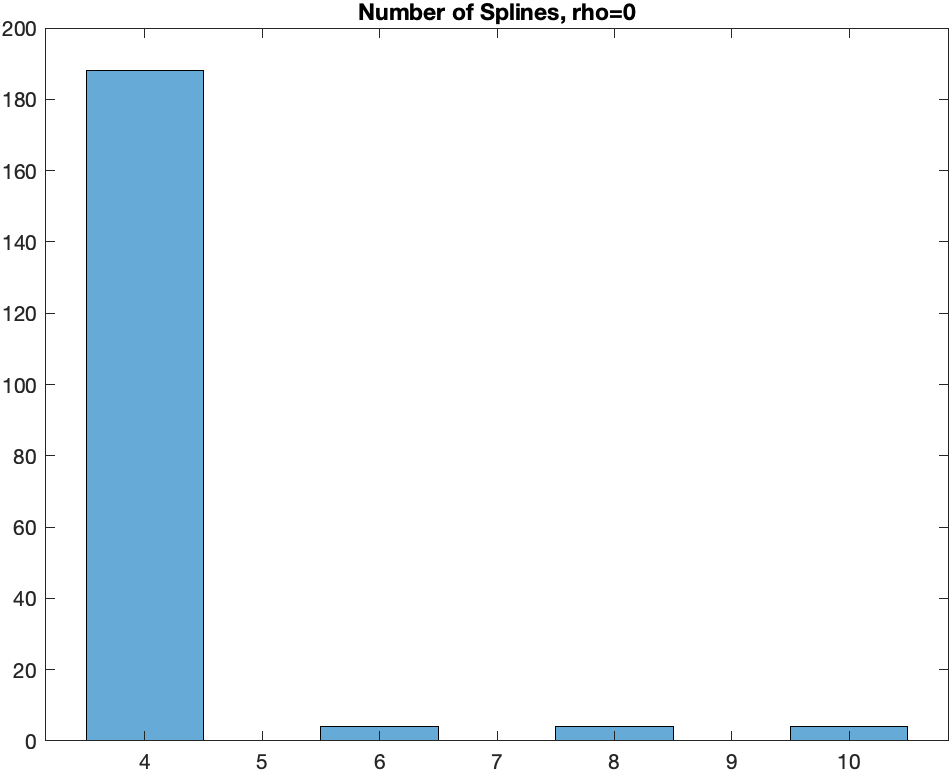
\includegraphics{../figures/hist_n_spli_rho-0_quadratic_splines.png}\end{minipage}%
%
\begin{minipage}{0.50\linewidth}
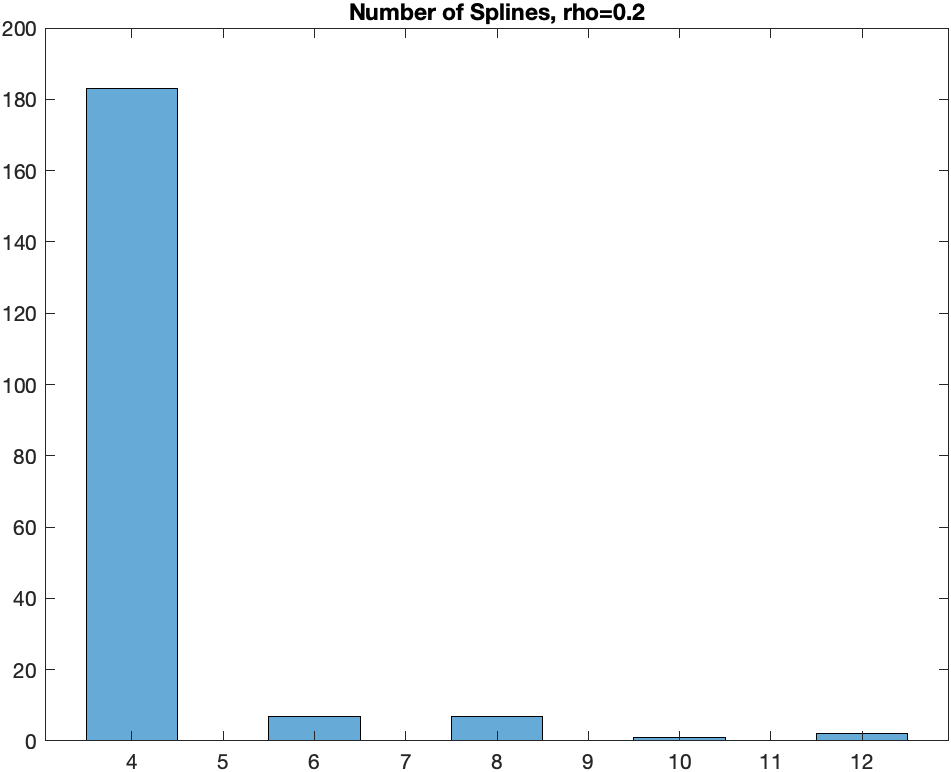
\includegraphics{../figures/hist_n_spli_rho-0.2_quadratic_splines.png}\end{minipage}%
\newline
\begin{minipage}{0.50\linewidth}
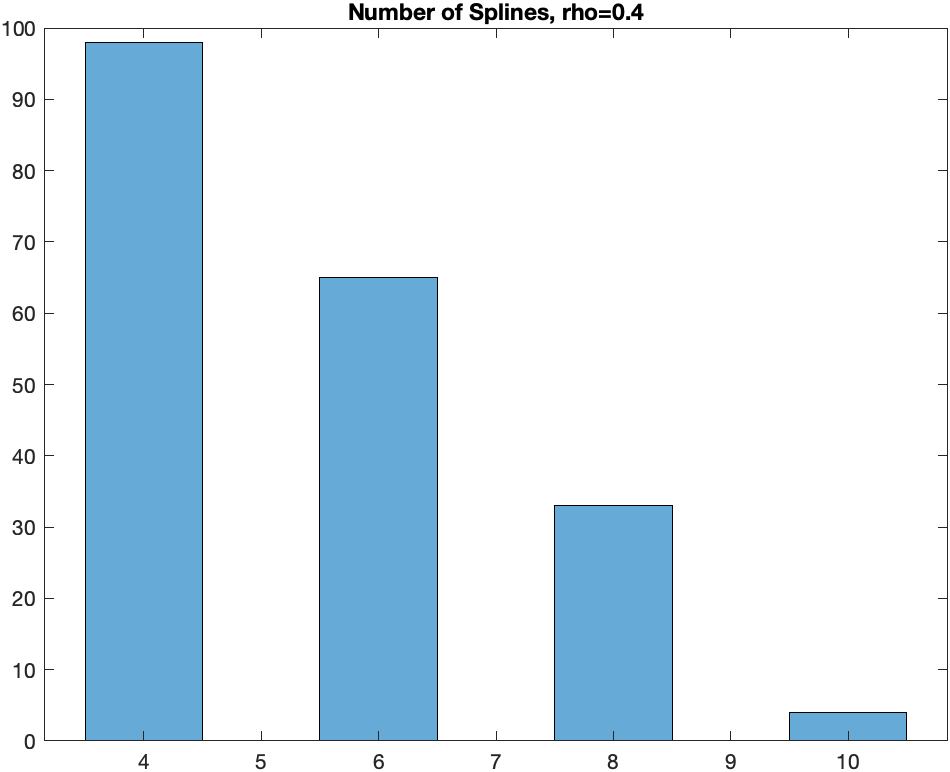
\includegraphics{../figures/hist_n_spli_rho-0.4_quadratic_splines.png}\end{minipage}%
%
\begin{minipage}{0.50\linewidth}
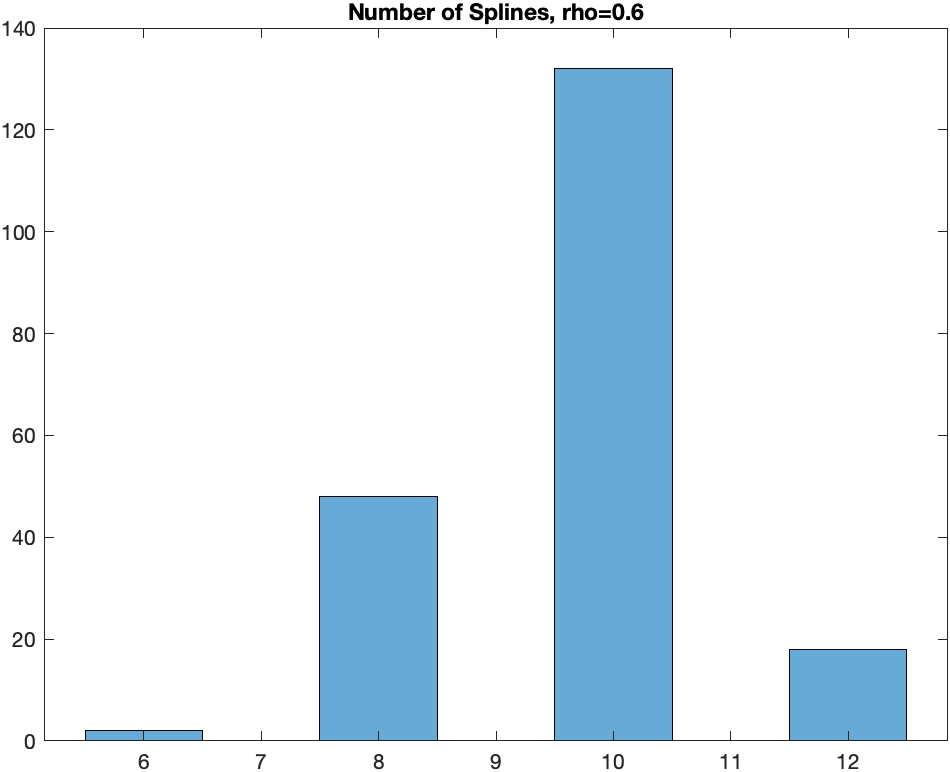
\includegraphics{../figures/hist_n_spli_rho-0.6_quadratic_splines.png}\end{minipage}%
\newline
\begin{minipage}{0.50\linewidth}
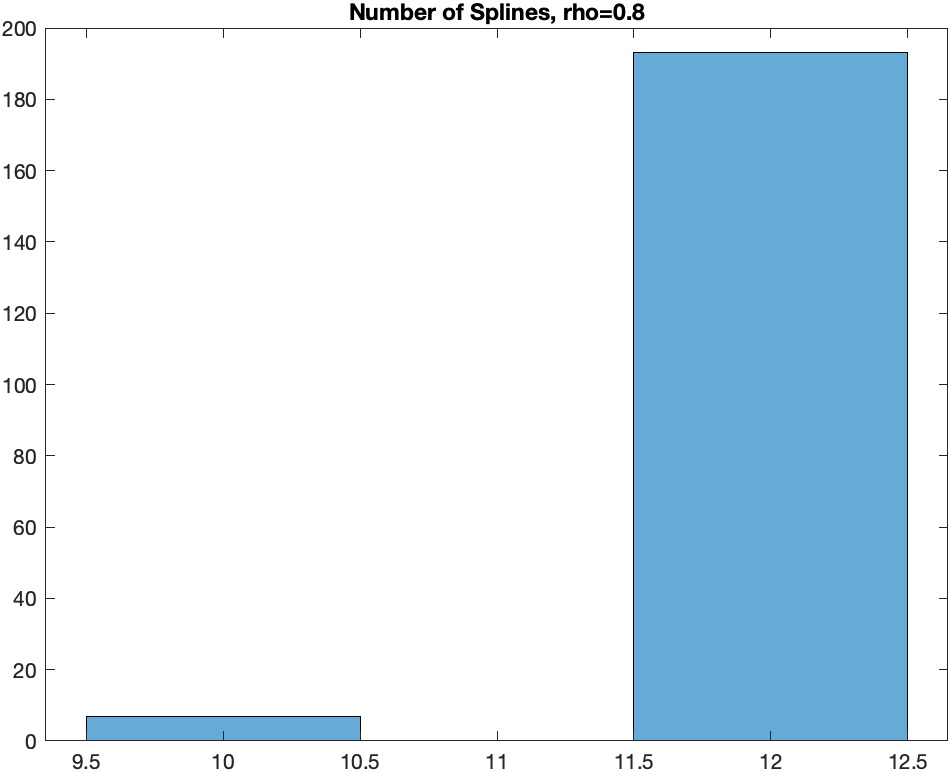
\includegraphics{../figures/hist_n_spli_rho-0.8_quadratic_splines.png}\end{minipage}%
%
\begin{minipage}{0.50\linewidth}
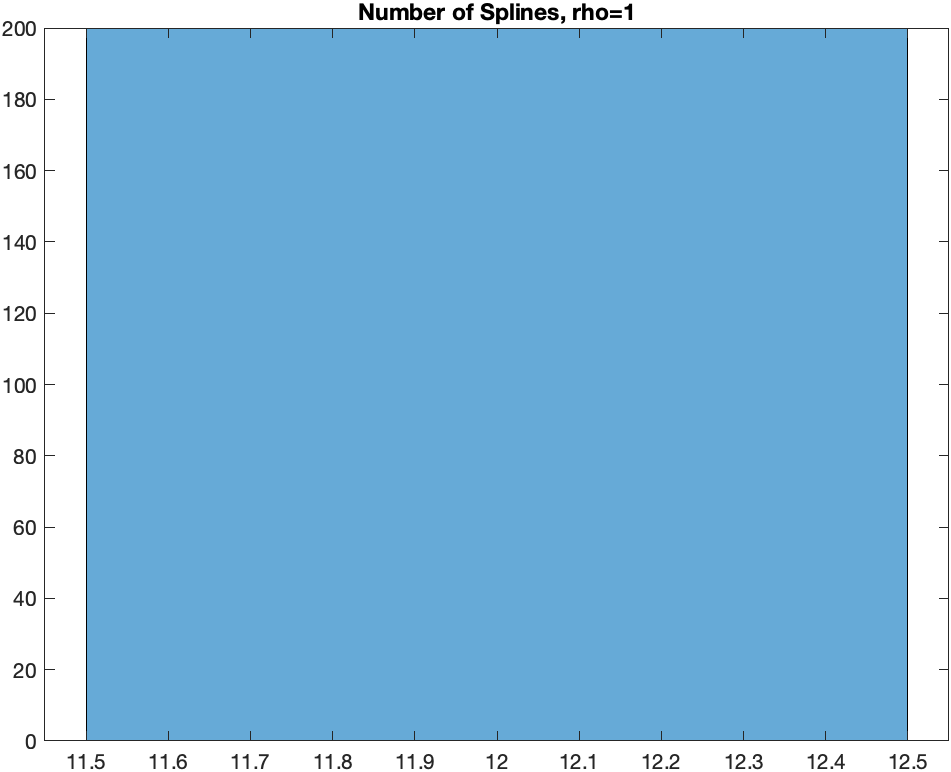
\includegraphics{../figures/hist_n_spli_rho-1_quadratic_splines.png}\end{minipage}%

\caption{\label{fig-hist-n-splies}Histograms of the number of quadratic
B-splines chosen by the level of \(\rho\)}

\end{figure}%

\section{8x8 Quadratic B-Spline}\label{sec-8x8}

Table~\ref{tbl-HAC-8x8} and Table~\ref{tbl-HAC-8x8-u} show the rejection
frequencies of testing the null hypothesis \(H_0=\hat\beta_0-\beta_0\)
for different values of \(\rho\) adding an 8x8 quadratic B-Spline for
the triangle and uniform kernel HAC.

Table~\ref{tbl-HAC-8x8-unif-bs} and Table~\ref{tbl-HAC-8x8-u-unif-bs}
show the same exercise but using an 8x8 step function B-Splines for the
triangle and uniform kernel HAC.

Table~\ref{tbl-HAC-8x8-ci} and Table~\ref{tbl-HAC-8x8-u-ci} show the
confidence interval lengths for the same simulations of tables
\ref{tbl-HAC-8x8} and \ref{tbl-HAC-8x8-u}. Likewise,
Table~\ref{tbl-HAC-8x8-ci-unif-bs} and
Table~\ref{tbl-HAC-8x8-u-ci-unif-bs} show the confidence interval
lengths for tables Table~\ref{tbl-HAC-8x8-unif-bs} and
Table~\ref{tbl-HAC-8x8-u-unif-bs}.

In addition, the tables show the rejection frequencies when using the
heteroscedastic robust variance for the standard error à la Stata and
the BIC.

BIC (Hansen 2020) is estimated as
\begin{equation}\phantomsection\label{eq-hansen-bic}{
BIC_H=T\log(2\pi\hat{\sigma}^2_{e_l})+T+(k+1)\log(T)
}\end{equation}

\begin{table}

\caption{\label{tbl-HAC-8x8}Rejection frequencies testing the null
hypothesis that the slope is statically different from the true value,
zero, using an 8x8 \textbf{quadratic} B-splines and the
\textbf{triangle} kernel HAC variance estimator for the standard error.
The number of B-splines was fixed at 8x8. 200 simulations. \textbf{500}
points. Column `corr' shows the theoretical correlation at distance
\(h=0.1\), thus, \(corr=\rho*\exp(-\frac{1}{\sqrt{2}})\). HR shows the
rejection frequencies of the Heteroscedastic Robust Variance estimator
(Stata's).}

\centering{

\begin{tabular}[t]{rrrrrrrrrrr}
\toprule
\multicolumn{11}{c}{Slope} \\
\cmidrule(l{3pt}r{3pt}){1-11}
\multicolumn{2}{c}{ } & \multicolumn{5}{c}{Tri-HAC+Quad-BS} \\
\cmidrule(l{3pt}r{3pt}){3-7}
...rho. & corr & 0.05 & 0.1 & 0.15 & 0.2 & 0.25 & NN & Drop & HR & BIC\\
\midrule
0.05 & 0.025 & 0.015 & 0.010 & 0.010 & 0.015 & 0.015 & -0.095 & 0 & 0.005 & 1707.970\\
0.15 & 0.074 & 0.035 & 0.035 & 0.035 & 0.040 & 0.040 & -0.069 & 0 & 0.035 & 1601.954\\
0.25 & 0.123 & 0.040 & 0.035 & 0.035 & 0.035 & 0.035 & -0.045 & 0 & 0.040 & 1486.763\\
0.35 & 0.173 & 0.050 & 0.050 & 0.055 & 0.055 & 0.055 & -0.025 & 0 & 0.090 & 1373.378\\
0.45 & 0.222 & 0.055 & 0.050 & 0.050 & 0.050 & 0.055 & -0.005 & 0 & 0.175 & 1259.761\\
\addlinespace
0.55 & 0.271 & 0.015 & 0.015 & 0.010 & 0.015 & 0.030 & 0.018 & 0 & 0.245 & 1150.565\\
0.65 & 0.320 & 0.060 & 0.065 & 0.065 & 0.070 & 0.070 & 0.042 & 0 & 0.385 & 1071.105\\
0.75 & 0.370 & 0.115 & 0.100 & 0.095 & 0.080 & 0.095 & 0.067 & 0 & 0.495 & 1036.040\\
0.85 & 0.419 & 0.165 & 0.155 & 0.140 & 0.130 & 0.120 & 0.093 & 0 & 0.490 & 1063.623\\
0.95 & 0.468 & 0.155 & 0.130 & 0.120 & 0.115 & 0.115 & 0.118 & 0 & 0.470 & 1128.922\\
\addlinespace
1.00 & 0.493 & 0.135 & 0.115 & 0.105 & 0.105 & 0.105 & 0.128 & 0 & 0.565 & 1165.828\\
\bottomrule
\end{tabular}

}

\end{table}%

\begin{table}

\caption{\label{tbl-HAC-8x8-u}Rejection frequencies testing the null
hypothesis that the slope is statically different from the true value,
zero, using an 8x8 \textbf{quadratic} B-splines and the \textbf{uniform}
kernel HAC variance estimator for the standard error. The number of
B-splines was fixed at 8x8. 200 simulations. \textbf{500} points. Column
`corr' shows the theoretical correlation at distance \(h=0.1\), thus,
\(corr=\rho*\exp(-\frac{1}{\sqrt{2}})\). HR shows the rejection
frequencies of the Heteroscedastic Robust Variance estimator (Stata's).}

\centering{

\begin{tabular}[t]{rrrrrrrrrrr}
\toprule
\multicolumn{11}{c}{Slope} \\
\cmidrule(l{3pt}r{3pt}){1-11}
\multicolumn{2}{c}{ } & \multicolumn{5}{c}{Unif-HAC+Quad-BS} \\
\cmidrule(l{3pt}r{3pt}){3-7}
...rho. & corr & 0.05 & 0.1 & 0.15 & 0.2 & 0.25 & NN & Drop & HR & BIC\\
\midrule
0.05 & 0.025 & 0.010 & 0.010 & 0.025 & 0.035 & 0.041 & -0.095 & 0 & 0.005 & 1707.970\\
0.15 & 0.074 & 0.030 & 0.045 & 0.045 & 0.090 & 0.113 & -0.069 & 0 & 0.035 & 1601.954\\
0.25 & 0.123 & 0.035 & 0.035 & 0.060 & 0.070 & 0.112 & -0.045 & 0 & 0.040 & 1486.763\\
0.35 & 0.173 & 0.050 & 0.060 & 0.060 & 0.080 & 0.106 & -0.025 & 0 & 0.090 & 1373.378\\
0.45 & 0.222 & 0.060 & 0.070 & 0.060 & 0.080 & 0.112 & -0.005 & 0 & 0.175 & 1259.761\\
\addlinespace
0.55 & 0.271 & 0.015 & 0.010 & 0.040 & 0.060 & 0.087 & 0.018 & 0 & 0.245 & 1150.565\\
0.65 & 0.320 & 0.065 & 0.075 & 0.085 & 0.095 & 0.117 & 0.042 & 0 & 0.385 & 1071.105\\
0.75 & 0.370 & 0.095 & 0.075 & 0.080 & 0.085 & 0.091 & 0.067 & 0 & 0.495 & 1036.040\\
0.85 & 0.419 & 0.145 & 0.135 & 0.110 & 0.140 & 0.126 & 0.093 & 0 & 0.490 & 1063.623\\
0.95 & 0.468 & 0.120 & 0.120 & 0.110 & 0.110 & 0.126 & 0.118 & 0 & 0.470 & 1128.922\\
\addlinespace
1.00 & 0.493 & 0.110 & 0.100 & 0.075 & 0.075 & 0.085 & 0.128 & 0 & 0.565 & 1165.828\\
\bottomrule
\end{tabular}

}

\end{table}%

\begin{table}

\caption{\label{tbl-HAC-8x8-unif-bs}Rejection frequencies testing the
null hypothesis that the slope is statically different from the true
value, zero, using an 8x8 \textbf{uniform} B-splines and the
\textbf{triangle} kernel HAC variance estimator for the standard error.
The number of B-splines was fixed at 8x8. 200 simulations. \textbf{500}
points. Column `corr' shows the theoretical correlation at distance
\(h=0.1\), thus, \(corr=\rho*\exp(-\frac{1}{\sqrt{2}})\). HR shows the
rejection frequencies of the Heteroscedastic Robust Variance estimator
(Stata's).}

\centering{

\begin{tabular}[t]{rrrrrrrrrrr}
\toprule
\multicolumn{11}{c}{Slope} \\
\cmidrule(l{3pt}r{3pt}){1-11}
\multicolumn{2}{c}{ } & \multicolumn{5}{c}{Tri-HAC+Unif-BS} \\
\cmidrule(l{3pt}r{3pt}){3-7}
...rho. & corr & 0.05 & 0.1 & 0.15 & 0.2 & 0.25 & NN & Drop & HR & BIC\\
\midrule
0.05 & 0.025 & 0.005 & 0.000 & 0.000 & 0.000 & 0.000 & -0.088 & 0 & 0.000 & 1708.773\\
0.15 & 0.074 & 0.050 & 0.045 & 0.040 & 0.045 & 0.050 & -0.067 & 0 & 0.035 & 1602.054\\
0.25 & 0.123 & 0.050 & 0.045 & 0.045 & 0.045 & 0.045 & -0.044 & 0 & 0.040 & 1488.871\\
0.35 & 0.173 & 0.045 & 0.040 & 0.045 & 0.045 & 0.050 & -0.023 & 0 & 0.090 & 1380.428\\
0.45 & 0.222 & 0.070 & 0.060 & 0.065 & 0.065 & 0.080 & -0.003 & 0 & 0.170 & 1273.005\\
\addlinespace
0.55 & 0.271 & 0.065 & 0.065 & 0.055 & 0.055 & 0.055 & 0.023 & 0 & 0.235 & 1180.528\\
0.65 & 0.320 & 0.115 & 0.115 & 0.100 & 0.095 & 0.095 & 0.044 & 0 & 0.380 & 1114.694\\
0.75 & 0.370 & 0.130 & 0.115 & 0.095 & 0.095 & 0.085 & 0.071 & 0 & 0.495 & 1095.898\\
0.85 & 0.419 & 0.175 & 0.155 & 0.130 & 0.110 & 0.110 & 0.097 & 0 & 0.480 & 1131.505\\
0.95 & 0.468 & 0.120 & 0.100 & 0.075 & 0.070 & 0.070 & 0.121 & 0 & 0.465 & 1202.925\\
\addlinespace
1.00 & 0.493 & 0.150 & 0.125 & 0.105 & 0.100 & 0.090 & 0.133 & 0 & 0.550 & 1244.951\\
\bottomrule
\end{tabular}

}

\end{table}%

\begin{table}

\caption{\label{tbl-HAC-8x8-u-unif-bs}Rejection frequencies testing the
null hypothesis that the slope is statically different from the true
value, zero, using an 8x8 \textbf{uniform} B-splines and the
\textbf{uniform} kernel HAC variance estimator for the standard error.
The number of B-splines was fixed at 8x8. 200 simulations. \textbf{500}
points. Column `corr' shows the theoretical correlation at distance
\(h=0.1\), thus, \(corr=\rho*\exp(-\frac{1}{\sqrt{2}})\). HR shows the
rejection frequencies of the Heteroscedastic Robust Variance estimator
(Stata's).}

\centering{

\begin{tabular}[t]{rrrrrrrrrrr}
\toprule
\multicolumn{11}{c}{Slope} \\
\cmidrule(l{3pt}r{3pt}){1-11}
\multicolumn{2}{c}{ } & \multicolumn{5}{c}{Unif-HAC+Unif-BS} \\
\cmidrule(l{3pt}r{3pt}){3-7}
...rho. & corr & 0.05 & 0.1 & 0.15 & 0.2 & 0.25 & NN & Drop & HR & BIC\\
\midrule
0.05 & 0.025 & 0.000 & 0.000 & 0.010 & 0.040 & 0.040 & -0.088 & 0 & 0.000 & 1708.773\\
0.15 & 0.074 & 0.045 & 0.040 & 0.050 & 0.065 & 0.095 & -0.067 & 0 & 0.035 & 1602.054\\
0.25 & 0.123 & 0.060 & 0.040 & 0.045 & 0.070 & 0.106 & -0.044 & 0 & 0.040 & 1488.871\\
0.35 & 0.173 & 0.040 & 0.055 & 0.055 & 0.080 & 0.092 & -0.023 & 0 & 0.090 & 1380.428\\
0.45 & 0.222 & 0.070 & 0.070 & 0.080 & 0.102 & 0.112 & -0.003 & 0 & 0.170 & 1273.005\\
\addlinespace
0.55 & 0.271 & 0.065 & 0.050 & 0.055 & 0.055 & 0.126 & 0.023 & 0 & 0.235 & 1180.528\\
0.65 & 0.320 & 0.115 & 0.095 & 0.090 & 0.116 & 0.152 & 0.044 & 0 & 0.380 & 1114.694\\
0.75 & 0.370 & 0.110 & 0.085 & 0.060 & 0.060 & 0.080 & 0.071 & 0 & 0.495 & 1095.898\\
0.85 & 0.419 & 0.155 & 0.115 & 0.115 & 0.115 & 0.120 & 0.097 & 0 & 0.480 & 1131.505\\
0.95 & 0.468 & 0.090 & 0.065 & 0.040 & 0.070 & 0.090 & 0.121 & 0 & 0.465 & 1202.925\\
\addlinespace
1.00 & 0.493 & 0.120 & 0.090 & 0.075 & 0.095 & 0.116 & 0.133 & 0 & 0.550 & 1244.951\\
\bottomrule
\end{tabular}

}

\end{table}%

\begin{table}

\caption{\label{tbl-HAC-8x8-ci}Confidence Interval length of using the
\textbf{triangle} kernel HAC variance estimator for the standard error
after adding an 8x8 \textbf{quadratic} B-splines. The number of
B-splines was fixed at 8x8. 200 simulations. \textbf{500} points. Column
`corr' shows the theoretical correlation at distance \(h=0.1\), thus,
\(corr=\rho*\exp(-\frac{1}{\sqrt{2}})\). HR shows the rejection
frequencies of the Heteroscedastic Robust Variance estimator (Stata's).}

\centering{

\begin{tabular}[t]{rrrrrrrrrrr}
\toprule
\multicolumn{11}{c}{Slope} \\
\cmidrule(l{3pt}r{3pt}){1-11}
\multicolumn{2}{c}{ } & \multicolumn{5}{c}{Tri-HAC+Quad-BS} \\
\cmidrule(l{3pt}r{3pt}){3-7}
...rho. & corr & 0.05 & 0.1 & 0.15 & 0.2 & 0.25 & NN & Drop & HR & BIC\\
\midrule
0.05 & 0.025 & 0.191 & 0.192 & 0.192 & 0.191 & 0.190 & -0.095 & 0 & 0.005 & 1707.970\\
0.15 & 0.074 & 0.190 & 0.191 & 0.192 & 0.192 & 0.191 & -0.069 & 0 & 0.035 & 1601.954\\
0.25 & 0.123 & 0.189 & 0.191 & 0.191 & 0.191 & 0.189 & -0.045 & 0 & 0.040 & 1486.763\\
0.35 & 0.173 & 0.191 & 0.192 & 0.192 & 0.191 & 0.189 & -0.025 & 0 & 0.090 & 1373.378\\
0.45 & 0.222 & 0.191 & 0.192 & 0.193 & 0.192 & 0.190 & -0.005 & 0 & 0.175 & 1259.761\\
\addlinespace
0.55 & 0.271 & 0.191 & 0.193 & 0.194 & 0.195 & 0.195 & 0.018 & 0 & 0.245 & 1150.565\\
0.65 & 0.320 & 0.197 & 0.200 & 0.203 & 0.205 & 0.205 & 0.042 & 0 & 0.385 & 1071.105\\
0.75 & 0.370 & 0.201 & 0.208 & 0.213 & 0.217 & 0.220 & 0.067 & 0 & 0.495 & 1036.040\\
0.85 & 0.419 & 0.211 & 0.221 & 0.229 & 0.234 & 0.238 & 0.093 & 0 & 0.490 & 1063.623\\
0.95 & 0.468 & 0.216 & 0.228 & 0.236 & 0.243 & 0.246 & 0.118 & 0 & 0.470 & 1128.922\\
\addlinespace
1.00 & 0.493 & 0.213 & 0.226 & 0.235 & 0.242 & 0.246 & 0.128 & 0 & 0.565 & 1165.828\\
\bottomrule
\end{tabular}

}

\end{table}%

\begin{table}

\caption{\label{tbl-HAC-8x8-u-ci}Confidence Interval length of using the
\textbf{uniform} kernel HAC variance estimator for the standard error
after adding an 8x8 \textbf{quadratic} B-splines. The number of
B-splines was fixed at 8x8. 200 simulations. \textbf{500} points. Column
`corr' shows the theoretical correlation at distance \(h=0.1\), thus,
\(corr=\rho*\exp(-\frac{1}{\sqrt{2}})\). HR shows the rejection
frequencies of the Heteroscedastic Robust Variance estimator (Stata's).}

\centering{

\begin{tabular}[t]{rrrrrrrrrrr}
\toprule
\multicolumn{11}{c}{Slope} \\
\cmidrule(l{3pt}r{3pt}){1-11}
\multicolumn{2}{c}{ } & \multicolumn{5}{c}{Unif-HAC+Quad-BS} \\
\cmidrule(l{3pt}r{3pt}){3-7}
...rho. & corr & 0.05 & 0.1 & 0.15 & 0.2 & 0.25 & NN & Drop & HR & BIC\\
\midrule
0.05 & 0.025 & 0.192 & 0.194 & 0.190 & 0.182 & 0.178 & -0.095 & 0 & 0.005 & 1707.970\\
0.15 & 0.074 & 0.192 & 0.193 & 0.192 & 0.185 & 0.182 & -0.069 & 0 & 0.035 & 1601.954\\
0.25 & 0.123 & 0.191 & 0.193 & 0.189 & 0.183 & 0.174 & -0.045 & 0 & 0.040 & 1486.763\\
0.35 & 0.173 & 0.192 & 0.192 & 0.189 & 0.183 & 0.176 & -0.025 & 0 & 0.090 & 1373.378\\
0.45 & 0.222 & 0.192 & 0.194 & 0.191 & 0.183 & 0.176 & -0.005 & 0 & 0.175 & 1259.761\\
\addlinespace
0.55 & 0.271 & 0.193 & 0.196 & 0.196 & 0.193 & 0.188 & 0.018 & 0 & 0.245 & 1150.565\\
0.65 & 0.320 & 0.201 & 0.205 & 0.211 & 0.208 & 0.202 & 0.042 & 0 & 0.385 & 1071.105\\
0.75 & 0.370 & 0.212 & 0.217 & 0.227 & 0.230 & 0.227 & 0.067 & 0 & 0.495 & 1036.040\\
0.85 & 0.419 & 0.227 & 0.237 & 0.250 & 0.252 & 0.249 & 0.093 & 0 & 0.490 & 1063.623\\
0.95 & 0.468 & 0.235 & 0.246 & 0.261 & 0.263 & 0.255 & 0.118 & 0 & 0.470 & 1128.922\\
\addlinespace
1.00 & 0.493 & 0.233 & 0.246 & 0.260 & 0.264 & 0.257 & 0.128 & 0 & 0.565 & 1165.828\\
\bottomrule
\end{tabular}

}

\end{table}%

\begin{table}

\caption{\label{tbl-HAC-8x8-ci-unif-bs}Confidence Interval length of
using the \textbf{triangle} kernel HAC variance estimator for the
standard error after adding an 8x8 \textbf{uniform} B-splines. The
number of B-splines was fixed at 8x8. 200 simulations. \textbf{500}
points. Column `corr' shows the theoretical correlation at distance
\(h=0.1\), thus, \(corr=\rho*\exp(-\frac{1}{\sqrt{2}})\). HR shows the
rejection frequencies of the Heteroscedastic Robust Variance estimator
(Stata's).}

\centering{

\begin{tabular}[t]{rrrrrrrrrrr}
\toprule
\multicolumn{11}{c}{Slope} \\
\cmidrule(l{3pt}r{3pt}){1-11}
\multicolumn{2}{c}{ } & \multicolumn{5}{c}{Tri-HAC+Quad-BS} \\
\cmidrule(l{3pt}r{3pt}){3-7}
...rho. & corr & 0.05 & 0.1 & 0.15 & 0.2 & 0.25 & NN & Drop & HR & BIC\\
\midrule
0.05 & 0.025 & 0.189 & 0.191 & 0.192 & 0.192 & 0.191 & -0.088 & 0 & 0.000 & 1708.773\\
0.15 & 0.074 & 0.188 & 0.190 & 0.192 & 0.192 & 0.191 & -0.067 & 0 & 0.035 & 1602.054\\
0.25 & 0.123 & 0.187 & 0.189 & 0.191 & 0.191 & 0.190 & -0.044 & 0 & 0.040 & 1488.871\\
0.35 & 0.173 & 0.189 & 0.191 & 0.192 & 0.192 & 0.191 & -0.023 & 0 & 0.090 & 1380.428\\
0.45 & 0.222 & 0.189 & 0.191 & 0.193 & 0.193 & 0.192 & -0.003 & 0 & 0.170 & 1273.005\\
\addlinespace
0.55 & 0.271 & 0.191 & 0.194 & 0.198 & 0.199 & 0.200 & 0.023 & 0 & 0.235 & 1180.528\\
0.65 & 0.320 & 0.195 & 0.200 & 0.206 & 0.210 & 0.211 & 0.044 & 0 & 0.380 & 1114.694\\
0.75 & 0.370 & 0.200 & 0.210 & 0.220 & 0.227 & 0.230 & 0.071 & 0 & 0.495 & 1095.898\\
0.85 & 0.419 & 0.211 & 0.223 & 0.235 & 0.243 & 0.247 & 0.097 & 0 & 0.480 & 1131.505\\
0.95 & 0.468 & 0.213 & 0.228 & 0.243 & 0.253 & 0.258 & 0.121 & 0 & 0.465 & 1202.925\\
\addlinespace
1.00 & 0.493 & 0.214 & 0.229 & 0.244 & 0.253 & 0.258 & 0.133 & 0 & 0.550 & 1244.951\\
\bottomrule
\end{tabular}

}

\end{table}%

\begin{table}

\caption{\label{tbl-HAC-8x8-u-ci-unif-bs}Confidence Interval length of
using the \textbf{uniform} kernel HAC variance estimator for the
standard error after adding an 8x8 \textbf{uniform} B-splines. The
number of B-splines was fixed at 8x8. 200 simulations. \textbf{500}
points. Column `corr' shows the theoretical correlation at distance
\(h=0.1\), thus, \(corr=\rho*\exp(-\frac{1}{\sqrt{2}})\). HR shows the
rejection frequencies of the Heteroscedastic Robust Variance estimator
(Stata's).}

\centering{

\begin{tabular}[t]{rrrrrrrrrrr}
\toprule
\multicolumn{11}{c}{Slope} \\
\cmidrule(l{3pt}r{3pt}){1-11}
\multicolumn{2}{c}{ } & \multicolumn{5}{c}{Unif-HAC+Quad-BS} \\
\cmidrule(l{3pt}r{3pt}){3-7}
...rho. & corr & 0.05 & 0.1 & 0.15 & 0.2 & 0.25 & NN & Drop & HR & BIC\\
\midrule
0.05 & 0.025 & 0.191 & 0.195 & 0.192 & 0.185 & 0.180 & -0.088 & 0 & 0.000 & 1708.773\\
0.15 & 0.074 & 0.190 & 0.195 & 0.194 & 0.188 & 0.182 & -0.067 & 0 & 0.035 & 1602.054\\
0.25 & 0.123 & 0.188 & 0.194 & 0.191 & 0.188 & 0.176 & -0.044 & 0 & 0.040 & 1488.871\\
0.35 & 0.173 & 0.190 & 0.194 & 0.195 & 0.187 & 0.183 & -0.023 & 0 & 0.090 & 1380.428\\
0.45 & 0.222 & 0.190 & 0.198 & 0.196 & 0.189 & 0.182 & -0.003 & 0 & 0.170 & 1273.005\\
\addlinespace
0.55 & 0.271 & 0.193 & 0.202 & 0.206 & 0.203 & 0.196 & 0.023 & 0 & 0.235 & 1180.528\\
0.65 & 0.320 & 0.199 & 0.213 & 0.224 & 0.220 & 0.210 & 0.044 & 0 & 0.380 & 1114.694\\
0.75 & 0.370 & 0.210 & 0.232 & 0.248 & 0.247 & 0.241 & 0.071 & 0 & 0.495 & 1095.898\\
0.85 & 0.419 & 0.224 & 0.250 & 0.268 & 0.266 & 0.258 & 0.097 & 0 & 0.480 & 1131.505\\
0.95 & 0.468 & 0.228 & 0.261 & 0.285 & 0.283 & 0.274 & 0.121 & 0 & 0.465 & 1202.925\\
\addlinespace
1.00 & 0.493 & 0.230 & 0.262 & 0.283 & 0.280 & 0.273 & 0.133 & 0 & 0.550 & 1244.951\\
\bottomrule
\end{tabular}

}

\end{table}%

\section{Non-Monotonicity}\label{sec-finer}

In this section, I use a finer grid going from 0.8 to 1 to investigate
the apparently non-monotonicity of the rejection frequencies.

Table~\ref{tbl-HAC-quad-BS-slope-finer} and
Table~\ref{tbl-HAC-quad-BS-slope-u-finer} show the rejection frequencies
using quadratic and uniforms B-Splines with uniform kernel HAC estimator
while Table~\ref{tbl-img-slope-quad-finer} and
Table~\ref{tbl-img-slope-u-quad-finer} display the average number of
imaginary S.E. during simulations.

Figure~\ref{fig-hist-n-splies-finer-8} and
Figure~\ref{fig-hist-n-splies-finer-9} show the distribution of the
number of splines chosen by level of \(\rho\).

\begin{table}

\caption{\label{tbl-HAC-quad-BS-slope-finer}Rejection frequencies
testing the null hypothesis that the slope is statically different from
the true value, zero, using \textbf{quadratic} B-splines and the
\textbf{triangle} kernel HAC variance estimator for the standard error.
The number of B-splines selected minimizes the nearest neighbor (NN)
correlation of the OLS residuals to 0.05. 200 simulations. \textbf{500}
points. Column `corr' shows the theoretical correlation at distance
\(h=0.1\), thus, \(corr=\rho*\exp(-\frac{1}{\sqrt{2}})\).}

\centering{

\begin{tabular}[t]{rrrrrrrrrrrr}
\toprule
\multicolumn{12}{c}{Slope} \\
\cmidrule(l{3pt}r{3pt}){1-12}
\multicolumn{2}{c}{ } & \multicolumn{8}{c}{Tri-HAC+Quad-BS} \\
\cmidrule(l{3pt}r{3pt}){3-10}
...rho. & corr & 0.05 & 0.1 & 0.15 & 0.2 & 0.25 & 0.3 & 0.35 & 0.4 & NN & Drop\\
\midrule
0.80 & 0.394 & 0.150 & 0.125 & 0.095 & 0.070 & 0.080 & 0.085 & 0.080 & 0.080 & 0.050 & 45.76\\
0.81 & 0.399 & 0.065 & 0.060 & 0.055 & 0.050 & 0.065 & 0.065 & 0.070 & 0.070 & 0.050 & 45.60\\
0.82 & 0.404 & 0.100 & 0.080 & 0.065 & 0.065 & 0.060 & 0.065 & 0.075 & 0.090 & 0.049 & 48.56\\
0.83 & 0.409 & 0.125 & 0.090 & 0.070 & 0.065 & 0.065 & 0.075 & 0.080 & 0.090 & 0.049 & 49.04\\
0.84 & 0.414 & 0.145 & 0.110 & 0.090 & 0.075 & 0.075 & 0.085 & 0.085 & 0.085 & 0.049 & 49.48\\
\addlinespace
0.85 & 0.419 & 0.160 & 0.125 & 0.100 & 0.085 & 0.085 & 0.085 & 0.095 & 0.105 & 0.050 & 49.44\\
0.86 & 0.424 & 0.115 & 0.110 & 0.090 & 0.085 & 0.080 & 0.085 & 0.085 & 0.090 & 0.051 & 51.20\\
0.87 & 0.429 & 0.120 & 0.090 & 0.070 & 0.065 & 0.065 & 0.070 & 0.075 & 0.080 & 0.048 & 51.68\\
0.88 & 0.434 & 0.125 & 0.105 & 0.105 & 0.095 & 0.090 & 0.085 & 0.085 & 0.085 & 0.049 & 52.64\\
0.89 & 0.439 & 0.125 & 0.115 & 0.110 & 0.095 & 0.085 & 0.090 & 0.090 & 0.090 & 0.051 & 52.08\\
\addlinespace
0.90 & 0.444 & 0.130 & 0.125 & 0.095 & 0.095 & 0.100 & 0.090 & 0.095 & 0.105 & 0.051 & 53.60\\
0.91 & 0.449 & 0.080 & 0.055 & 0.050 & 0.055 & 0.065 & 0.070 & 0.075 & 0.080 & 0.052 & 53.84\\
0.92 & 0.454 & 0.140 & 0.120 & 0.095 & 0.090 & 0.085 & 0.080 & 0.080 & 0.075 & 0.051 & 53.92\\
0.93 & 0.459 & 0.130 & 0.110 & 0.095 & 0.090 & 0.095 & 0.095 & 0.090 & 0.090 & 0.054 & 53.68\\
0.94 & 0.463 & 0.145 & 0.120 & 0.105 & 0.110 & 0.110 & 0.110 & 0.110 & 0.125 & 0.055 & 54.48\\
\addlinespace
0.95 & 0.468 & 0.145 & 0.115 & 0.090 & 0.085 & 0.080 & 0.095 & 0.090 & 0.095 & 0.056 & 54.48\\
0.96 & 0.473 & 0.100 & 0.080 & 0.060 & 0.060 & 0.060 & 0.055 & 0.060 & 0.060 & 0.057 & 54.80\\
0.97 & 0.478 & 0.145 & 0.115 & 0.095 & 0.085 & 0.095 & 0.095 & 0.095 & 0.095 & 0.056 & 55.20\\
0.98 & 0.483 & 0.125 & 0.085 & 0.060 & 0.065 & 0.065 & 0.080 & 0.080 & 0.085 & 0.056 & 54.88\\
0.99 & 0.488 & 0.110 & 0.090 & 0.085 & 0.080 & 0.080 & 0.085 & 0.095 & 0.095 & 0.060 & 55.44\\
\addlinespace
1.00 & 0.493 & 0.165 & 0.130 & 0.115 & 0.105 & 0.110 & 0.110 & 0.120 & 0.130 & 0.061 & 55.28\\
\bottomrule
\end{tabular}

}

\end{table}%

\begin{table}

\caption{\label{tbl-img-slope-quad-finer}Share of imaginary se in
simulations for HAC+Quadratic Bsplines. Slope.}

\centering{

\begin{tabular}[t]{rrrrrrrrrrrr}
\toprule
\multicolumn{12}{c}{Slope} \\
\cmidrule(l{3pt}r{3pt}){1-12}
\multicolumn{2}{c}{ } & \multicolumn{8}{c}{Tri-HAC+Quad-BS} \\
\cmidrule(l{3pt}r{3pt}){3-10}
...rho. & corr & 0.05 & 0.1 & 0.15 & 0.2 & 0.25 & 0.3 & 0.35 & 0.4 & NN & Drop\\
\midrule
0.80 & 0.394 & 0 & 0 & 0 & 0 & 0 & 0 & 0 & 0 & 0.050 & 45.76\\
0.81 & 0.399 & 0 & 0 & 0 & 0 & 0 & 0 & 0 & 0 & 0.050 & 45.60\\
0.82 & 0.404 & 0 & 0 & 0 & 0 & 0 & 0 & 0 & 0 & 0.049 & 48.56\\
0.83 & 0.409 & 0 & 0 & 0 & 0 & 0 & 0 & 0 & 0 & 0.049 & 49.04\\
0.84 & 0.414 & 0 & 0 & 0 & 0 & 0 & 0 & 0 & 0 & 0.049 & 49.48\\
\addlinespace
0.85 & 0.419 & 0 & 0 & 0 & 0 & 0 & 0 & 0 & 0 & 0.050 & 49.44\\
0.86 & 0.424 & 0 & 0 & 0 & 0 & 0 & 0 & 0 & 0 & 0.051 & 51.20\\
0.87 & 0.429 & 0 & 0 & 0 & 0 & 0 & 0 & 0 & 0 & 0.048 & 51.68\\
0.88 & 0.434 & 0 & 0 & 0 & 0 & 0 & 0 & 0 & 0 & 0.049 & 52.64\\
0.89 & 0.439 & 0 & 0 & 0 & 0 & 0 & 0 & 0 & 0 & 0.051 & 52.08\\
\addlinespace
0.90 & 0.444 & 0 & 0 & 0 & 0 & 0 & 0 & 0 & 0 & 0.051 & 53.60\\
0.91 & 0.449 & 0 & 0 & 0 & 0 & 0 & 0 & 0 & 0 & 0.052 & 53.84\\
0.92 & 0.454 & 0 & 0 & 0 & 0 & 0 & 0 & 0 & 0 & 0.051 & 53.92\\
0.93 & 0.459 & 0 & 0 & 0 & 0 & 0 & 0 & 0 & 0 & 0.054 & 53.68\\
0.94 & 0.463 & 0 & 0 & 0 & 0 & 0 & 0 & 0 & 0 & 0.055 & 54.48\\
\addlinespace
0.95 & 0.468 & 0 & 0 & 0 & 0 & 0 & 0 & 0 & 0 & 0.056 & 54.48\\
0.96 & 0.473 & 0 & 0 & 0 & 0 & 0 & 0 & 0 & 0 & 0.057 & 54.80\\
0.97 & 0.478 & 0 & 0 & 0 & 0 & 0 & 0 & 0 & 0 & 0.056 & 55.20\\
0.98 & 0.483 & 0 & 0 & 0 & 0 & 0 & 0 & 0 & 0 & 0.056 & 54.88\\
0.99 & 0.488 & 0 & 0 & 0 & 0 & 0 & 0 & 0 & 0 & 0.060 & 55.44\\
\addlinespace
1.00 & 0.493 & 0 & 0 & 0 & 0 & 0 & 0 & 0 & 0 & 0.061 & 55.28\\
\bottomrule
\end{tabular}

}

\end{table}%

\begin{table}

\caption{\label{tbl-HAC-quad-BS-slope-u-finer}Rejection frequencies
testing the null hypothesis that the slope is statically different from
the true value, zero, using B-splines and the \textbf{uniform} kernel
HAC variance estimator for the standard error. The number of
\textbf{quadratic} B-splines selected minimizes the nearest neighbor
(NN) correlation of the OLS residuals to 0.05. 200 simulations.
\textbf{500} points. Column `corr' shows the theoretical correlation at
distance \(h=0.1\), thus, \(corr=\rho*\exp(-\frac{1}{\sqrt{2}})\).}

\centering{

\begin{tabular}[t]{rrrrrrrrrrrr}
\toprule
\multicolumn{12}{c}{Slope} \\
\cmidrule(l{3pt}r{3pt}){1-12}
\multicolumn{2}{c}{ } & \multicolumn{8}{c}{Unif-HAC+Quad-BS} \\
\cmidrule(l{3pt}r{3pt}){3-10}
...rho. & corr & 0.05 & 0.1 & 0.15 & 0.2 & 0.25 & 0.3 & 0.35 & 0.4 & NN & Drop\\
\midrule
0.80 & 0.394 & 0.130 & 0.065 & 0.060 & 0.070 & 0.085 & 0.107 & 0.147 & 0.196 & 0.050 & 45.76\\
0.81 & 0.399 & 0.065 & 0.050 & 0.060 & 0.070 & 0.095 & 0.118 & 0.115 & 0.134 & 0.050 & 45.60\\
0.82 & 0.404 & 0.085 & 0.040 & 0.065 & 0.080 & 0.100 & 0.129 & 0.139 & 0.144 & 0.049 & 48.56\\
0.83 & 0.409 & 0.090 & 0.055 & 0.070 & 0.070 & 0.081 & 0.127 & 0.160 & 0.156 & 0.049 & 49.04\\
0.84 & 0.414 & 0.115 & 0.065 & 0.070 & 0.080 & 0.111 & 0.146 & 0.177 & 0.132 & 0.049 & 49.48\\
\addlinespace
0.85 & 0.419 & 0.145 & 0.080 & 0.070 & 0.090 & 0.096 & 0.128 & 0.161 & 0.174 & 0.050 & 49.44\\
0.86 & 0.424 & 0.115 & 0.075 & 0.075 & 0.080 & 0.085 & 0.111 & 0.138 & 0.148 & 0.051 & 51.20\\
0.87 & 0.429 & 0.095 & 0.050 & 0.055 & 0.080 & 0.101 & 0.128 & 0.150 & 0.152 & 0.048 & 51.68\\
0.88 & 0.434 & 0.120 & 0.075 & 0.080 & 0.095 & 0.096 & 0.135 & 0.153 & 0.178 & 0.049 & 52.64\\
0.89 & 0.439 & 0.120 & 0.065 & 0.050 & 0.090 & 0.096 & 0.136 & 0.162 & 0.180 & 0.051 & 52.08\\
\addlinespace
0.90 & 0.444 & 0.130 & 0.080 & 0.080 & 0.100 & 0.121 & 0.141 & 0.159 & 0.214 & 0.051 & 53.60\\
0.91 & 0.449 & 0.070 & 0.045 & 0.060 & 0.075 & 0.115 & 0.124 & 0.144 & 0.157 & 0.052 & 53.84\\
0.92 & 0.454 & 0.120 & 0.085 & 0.080 & 0.090 & 0.116 & 0.148 & 0.132 & 0.155 & 0.051 & 53.92\\
0.93 & 0.459 & 0.115 & 0.075 & 0.075 & 0.095 & 0.110 & 0.120 & 0.149 & 0.168 & 0.054 & 53.68\\
0.94 & 0.463 & 0.120 & 0.100 & 0.090 & 0.100 & 0.116 & 0.160 & 0.168 & 0.200 & 0.055 & 54.48\\
\addlinespace
0.95 & 0.468 & 0.130 & 0.075 & 0.065 & 0.106 & 0.096 & 0.122 & 0.128 & 0.156 & 0.056 & 54.48\\
0.96 & 0.473 & 0.090 & 0.050 & 0.040 & 0.045 & 0.076 & 0.102 & 0.104 & 0.123 & 0.057 & 54.80\\
0.97 & 0.478 & 0.130 & 0.070 & 0.080 & 0.101 & 0.116 & 0.138 & 0.167 & 0.222 & 0.056 & 55.20\\
0.98 & 0.483 & 0.100 & 0.040 & 0.070 & 0.090 & 0.125 & 0.126 & 0.151 & 0.170 & 0.056 & 54.88\\
0.99 & 0.488 & 0.090 & 0.045 & 0.050 & 0.075 & 0.101 & 0.129 & 0.174 & 0.202 & 0.060 & 55.44\\
\addlinespace
1.00 & 0.493 & 0.150 & 0.080 & 0.100 & 0.120 & 0.121 & 0.144 & 0.179 & 0.223 & 0.061 & 55.28\\
\bottomrule
\end{tabular}

}

\end{table}%

\begin{table}

\caption{\label{tbl-img-slope-u-quad-finer}Share of imaginary se in
simulations for HAC+Quadratic Bsplines. Slope. Uniform Kernel HAC.}

\centering{

\begin{tabular}[t]{rrrrrrrrrrrr}
\toprule
\multicolumn{12}{c}{Slope} \\
\cmidrule(l{3pt}r{3pt}){1-12}
\multicolumn{2}{c}{ } & \multicolumn{8}{c}{Unif-HAC+Quad-BS} \\
\cmidrule(l{3pt}r{3pt}){3-10}
...rho. & corr & 0.05 & 0.1 & 0.15 & 0.2 & 0.25 & 0.3 & 0.35 & 0.4 & NN & Drop\\
\midrule
0.80 & 0.394 & 0 & 0 & 0 & 0.000 & 0.005 & 0.020 & 0.045 & 0.080 & 0.050 & 45.76\\
0.81 & 0.399 & 0 & 0 & 0 & 0.000 & 0.000 & 0.025 & 0.040 & 0.065 & 0.050 & 45.60\\
0.82 & 0.404 & 0 & 0 & 0 & 0.000 & 0.000 & 0.030 & 0.065 & 0.095 & 0.049 & 48.56\\
0.83 & 0.409 & 0 & 0 & 0 & 0.005 & 0.015 & 0.015 & 0.065 & 0.100 & 0.049 & 49.04\\
0.84 & 0.414 & 0 & 0 & 0 & 0.000 & 0.010 & 0.040 & 0.070 & 0.090 & 0.049 & 49.48\\
\addlinespace
0.85 & 0.419 & 0 & 0 & 0 & 0.000 & 0.010 & 0.025 & 0.040 & 0.080 & 0.050 & 49.44\\
0.86 & 0.424 & 0 & 0 & 0 & 0.005 & 0.005 & 0.010 & 0.025 & 0.085 & 0.051 & 51.20\\
0.87 & 0.429 & 0 & 0 & 0 & 0.000 & 0.005 & 0.025 & 0.035 & 0.110 & 0.048 & 51.68\\
0.88 & 0.434 & 0 & 0 & 0 & 0.000 & 0.010 & 0.035 & 0.055 & 0.045 & 0.049 & 52.64\\
0.89 & 0.439 & 0 & 0 & 0 & 0.000 & 0.010 & 0.010 & 0.045 & 0.085 & 0.051 & 52.08\\
\addlinespace
0.90 & 0.444 & 0 & 0 & 0 & 0.000 & 0.005 & 0.010 & 0.025 & 0.090 & 0.051 & 53.60\\
0.91 & 0.449 & 0 & 0 & 0 & 0.000 & 0.000 & 0.035 & 0.065 & 0.075 & 0.052 & 53.84\\
0.92 & 0.454 & 0 & 0 & 0 & 0.005 & 0.010 & 0.020 & 0.055 & 0.065 & 0.051 & 53.92\\
0.93 & 0.459 & 0 & 0 & 0 & 0.000 & 0.000 & 0.000 & 0.030 & 0.080 & 0.054 & 53.68\\
0.94 & 0.463 & 0 & 0 & 0 & 0.000 & 0.005 & 0.030 & 0.080 & 0.100 & 0.055 & 54.48\\
\addlinespace
0.95 & 0.468 & 0 & 0 & 0 & 0.010 & 0.015 & 0.020 & 0.065 & 0.070 & 0.056 & 54.48\\
0.96 & 0.473 & 0 & 0 & 0 & 0.000 & 0.010 & 0.015 & 0.040 & 0.065 & 0.057 & 54.80\\
0.97 & 0.478 & 0 & 0 & 0 & 0.005 & 0.005 & 0.020 & 0.040 & 0.100 & 0.056 & 55.20\\
0.98 & 0.483 & 0 & 0 & 0 & 0.000 & 0.000 & 0.050 & 0.070 & 0.120 & 0.056 & 54.88\\
0.99 & 0.488 & 0 & 0 & 0 & 0.000 & 0.005 & 0.030 & 0.050 & 0.085 & 0.060 & 55.44\\
\addlinespace
1.00 & 0.493 & 0 & 0 & 0 & 0.000 & 0.010 & 0.025 & 0.025 & 0.060 & 0.061 & 55.28\\
\bottomrule
\end{tabular}

}

\end{table}%

\begin{figure}

\begin{minipage}{0.50\linewidth}
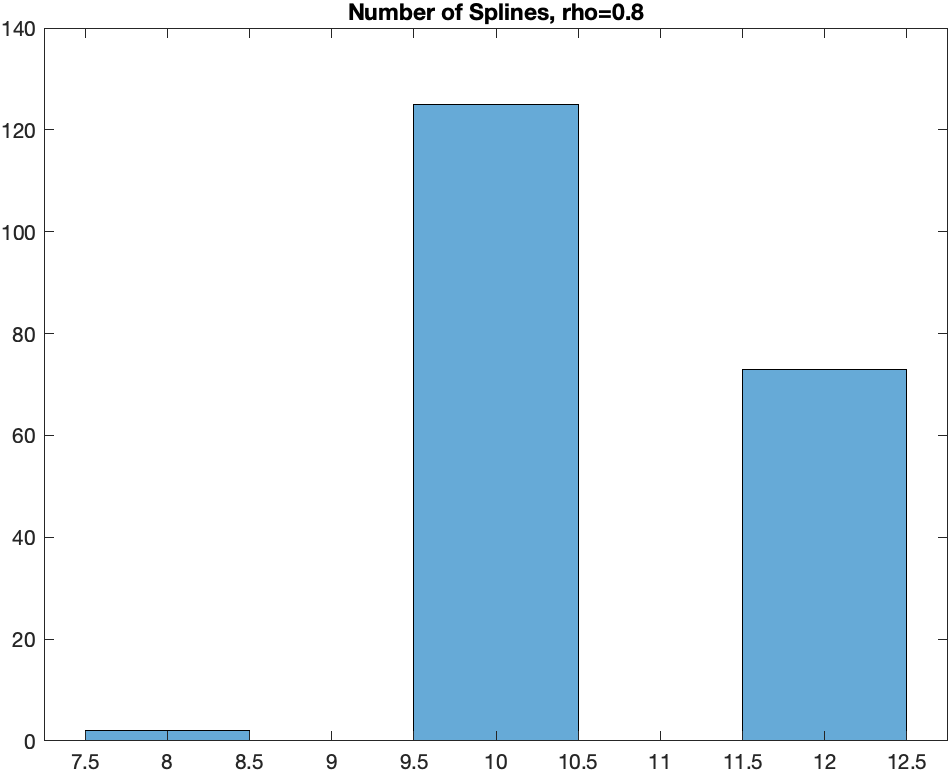
\includegraphics{../figures/hist_n_spli_rho-0.8_finer_grid.png}\end{minipage}%
%
\begin{minipage}{0.50\linewidth}
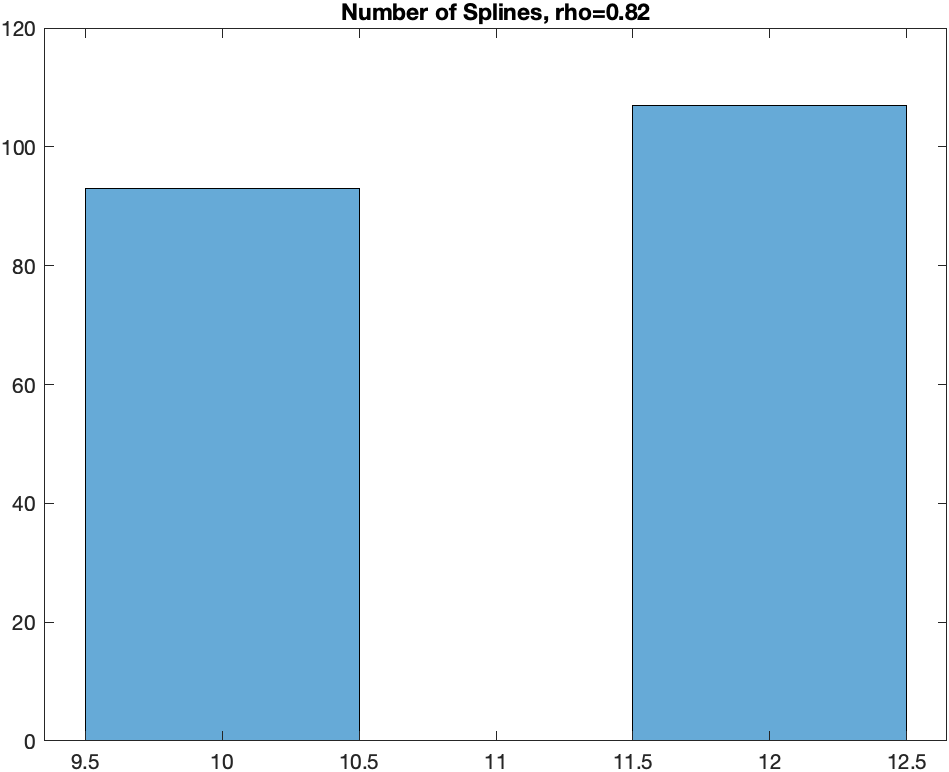
\includegraphics{../figures/hist_n_spli_rho-0.82_finer_grid.png}\end{minipage}%
\newline
\begin{minipage}{0.50\linewidth}
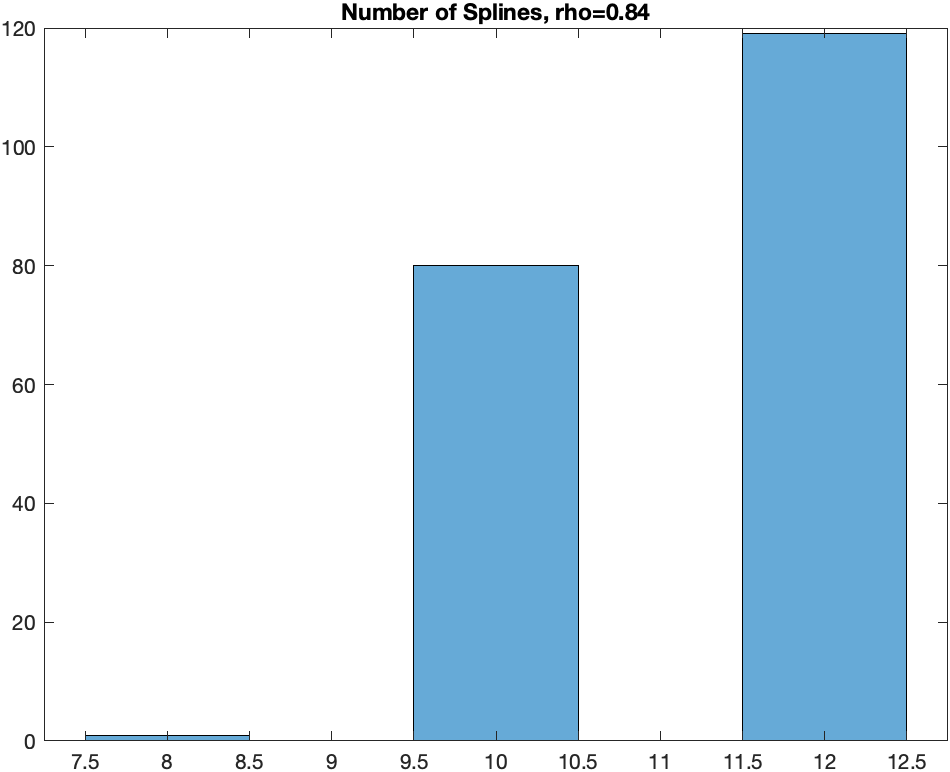
\includegraphics{../figures/hist_n_spli_rho-0.84_finer_grid.png}\end{minipage}%
%
\begin{minipage}{0.50\linewidth}
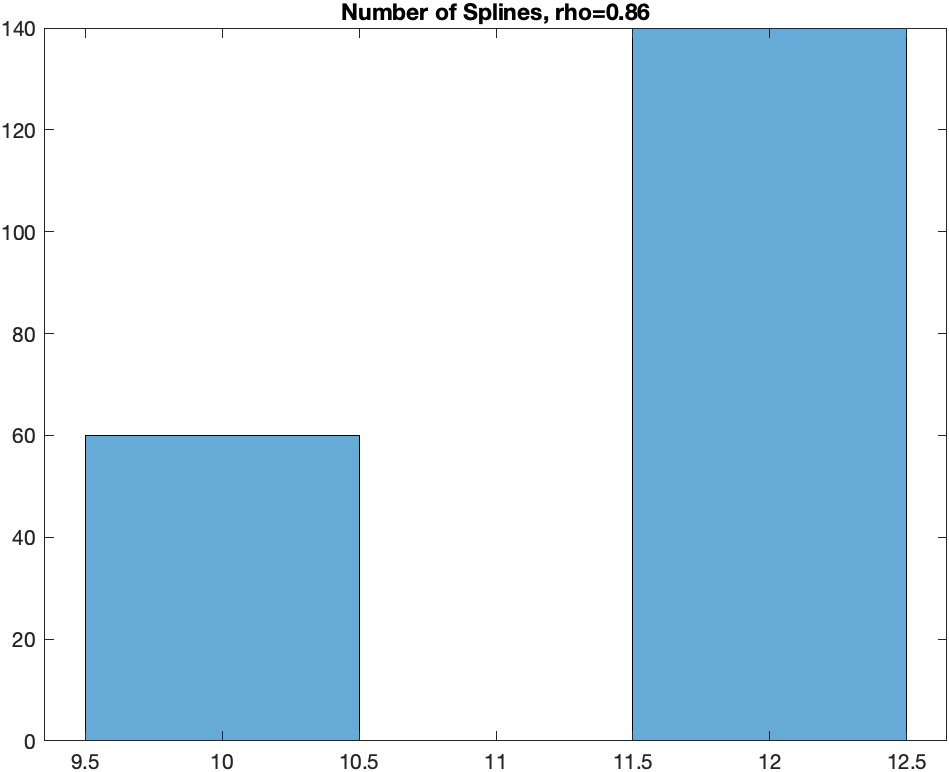
\includegraphics{../figures/hist_n_spli_rho-0.86_finer_grid.png}\end{minipage}%
\newline
\begin{minipage}{0.50\linewidth}
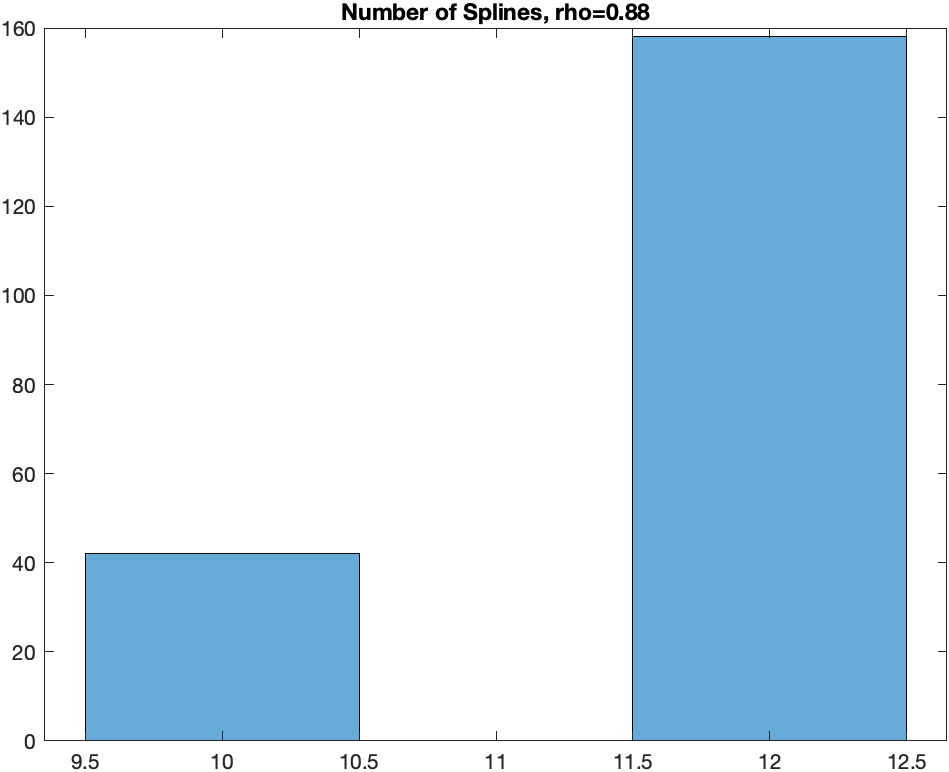
\includegraphics{../figures/hist_n_spli_rho-0.88_finer_grid.png}\end{minipage}%
%
\begin{minipage}{0.50\linewidth}
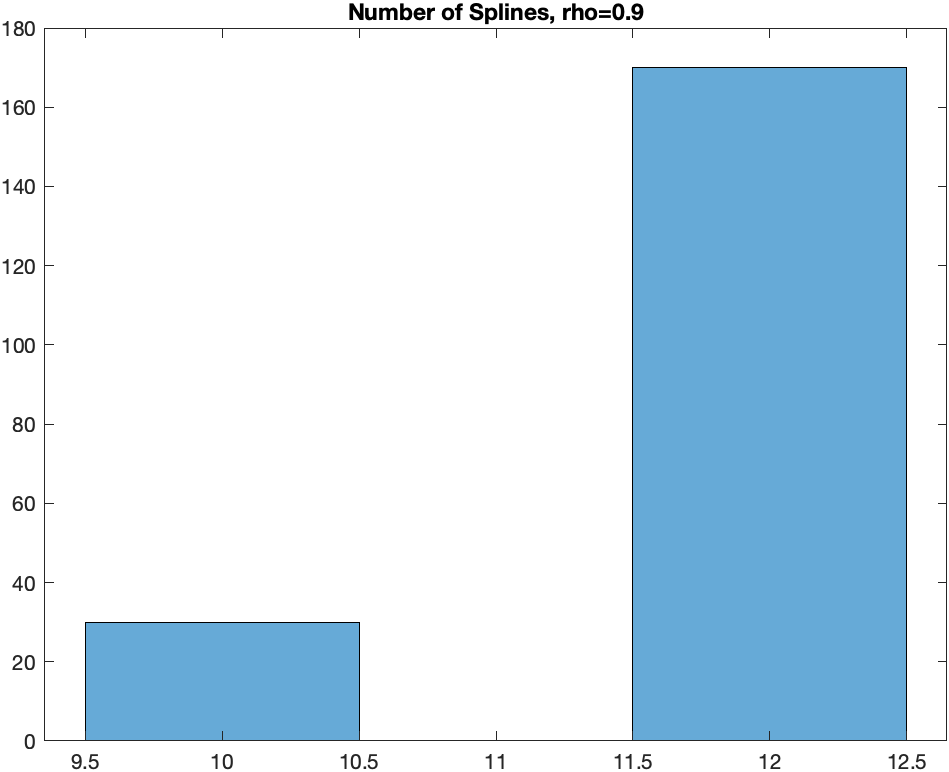
\includegraphics{../figures/hist_n_spli_rho-0.9_finer_grid.png}\end{minipage}%

\caption{\label{fig-hist-n-splies-finer-8}Histograms of the number of
quadratic B-splines chosen by the level of \(\rho\)}

\end{figure}%

\begin{figure}

\begin{minipage}{0.50\linewidth}
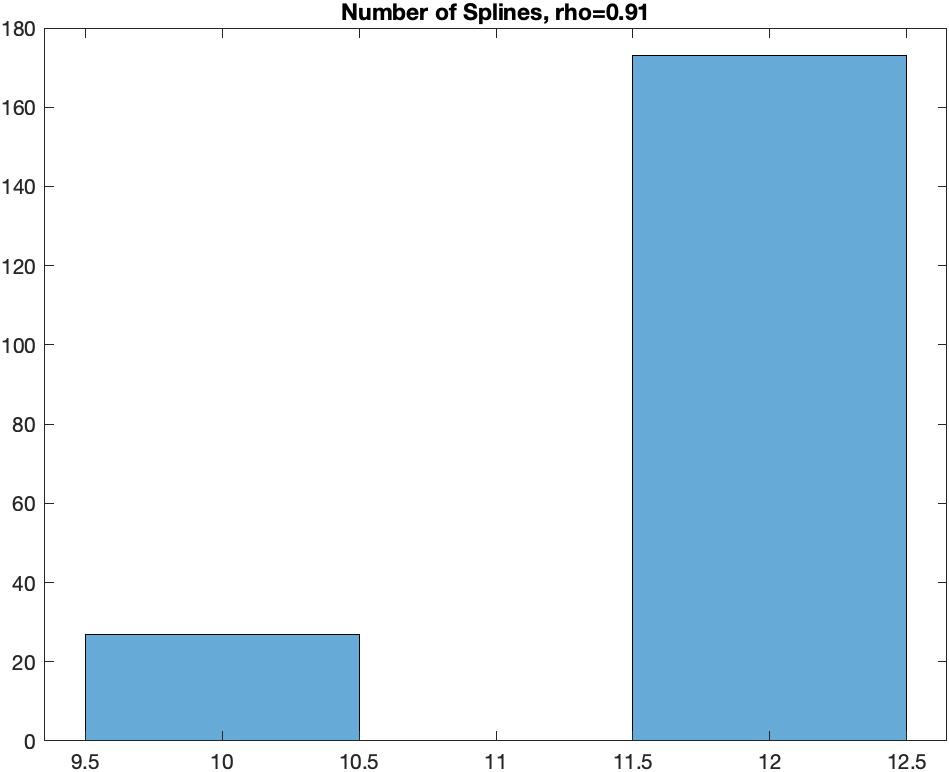
\includegraphics{../figures/hist_n_spli_rho-0.91_finer_grid.png}\end{minipage}%
%
\begin{minipage}{0.50\linewidth}
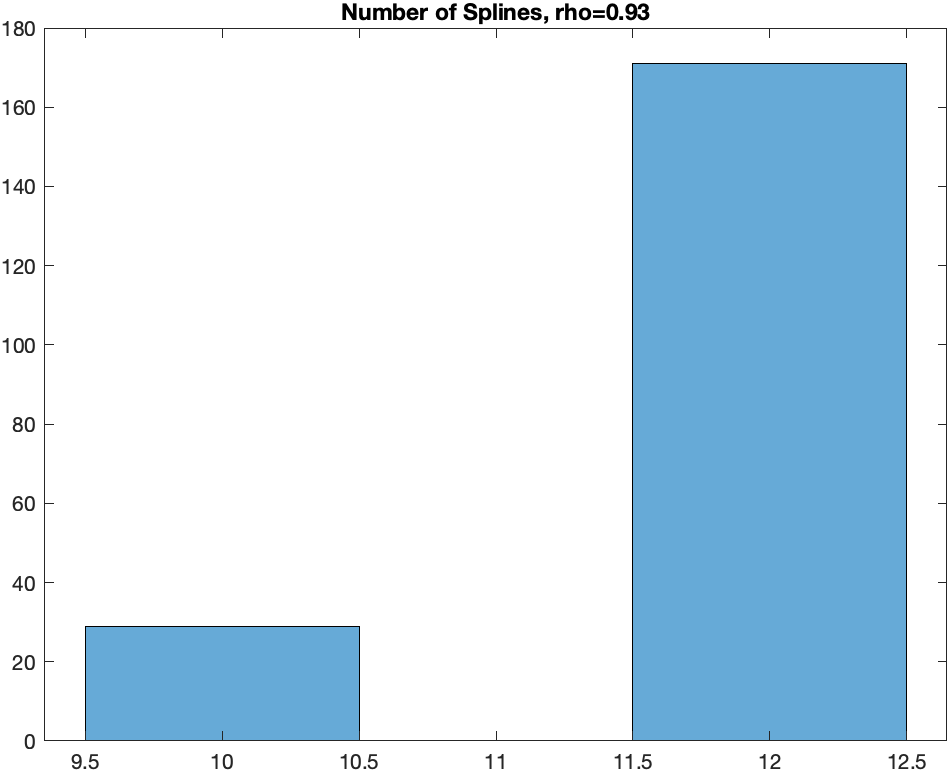
\includegraphics{../figures/hist_n_spli_rho-0.93_finer_grid.png}\end{minipage}%
\newline
\begin{minipage}{0.50\linewidth}
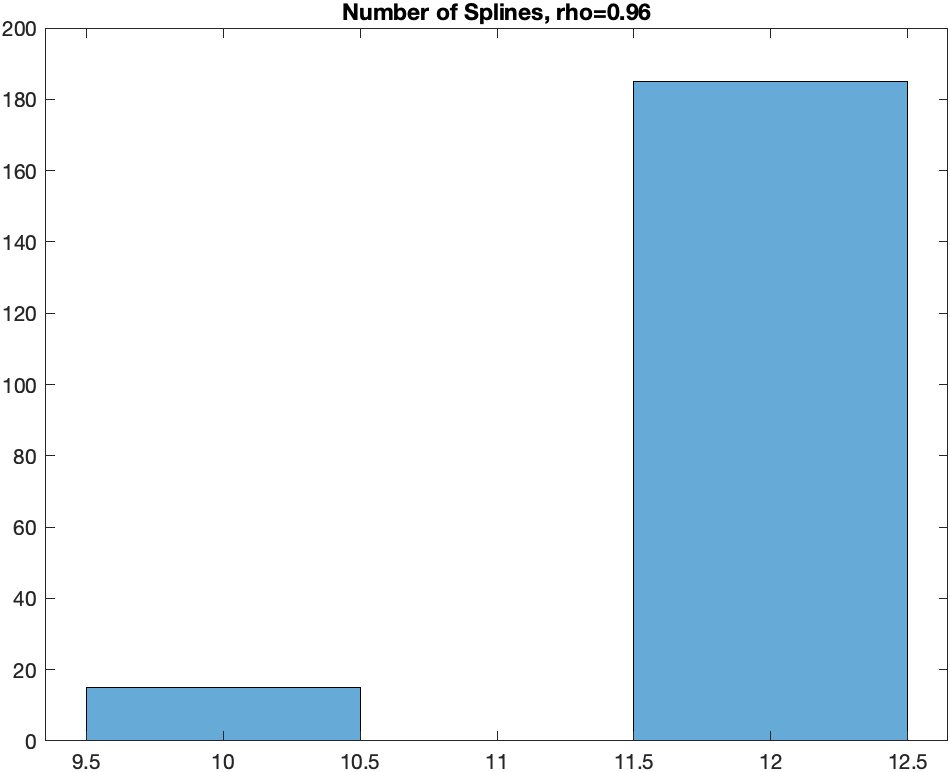
\includegraphics{../figures/hist_n_spli_rho-0.96_finer_grid.png}\end{minipage}%
%
\begin{minipage}{0.50\linewidth}
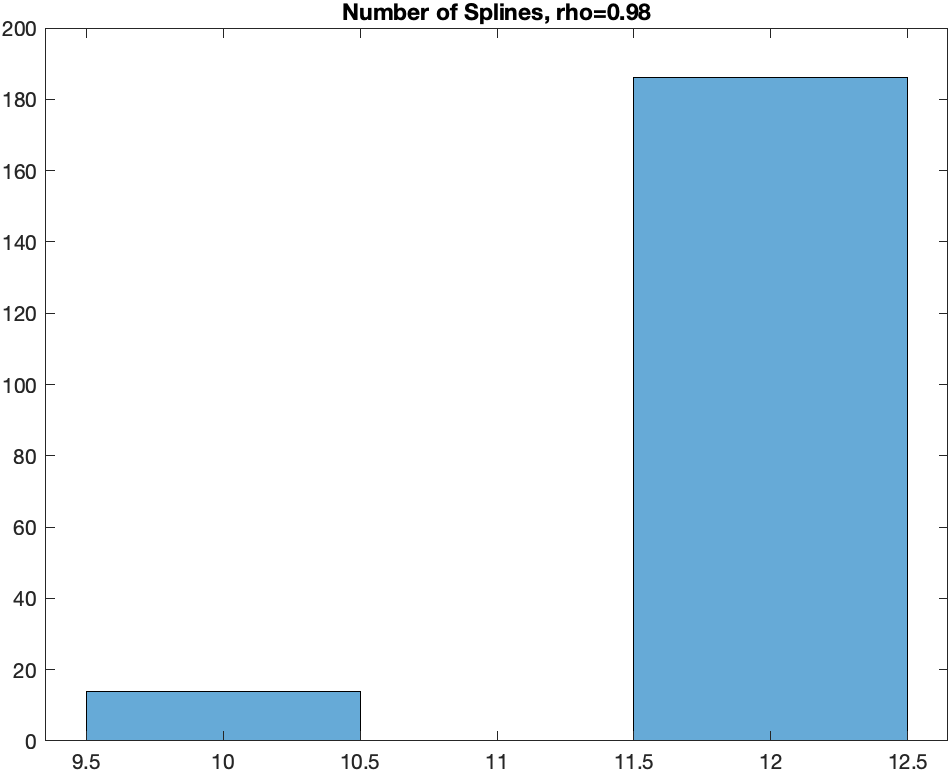
\includegraphics{../figures/hist_n_spli_rho-0.98_finer_grid.png}\end{minipage}%
\newline
\begin{minipage}{0.50\linewidth}
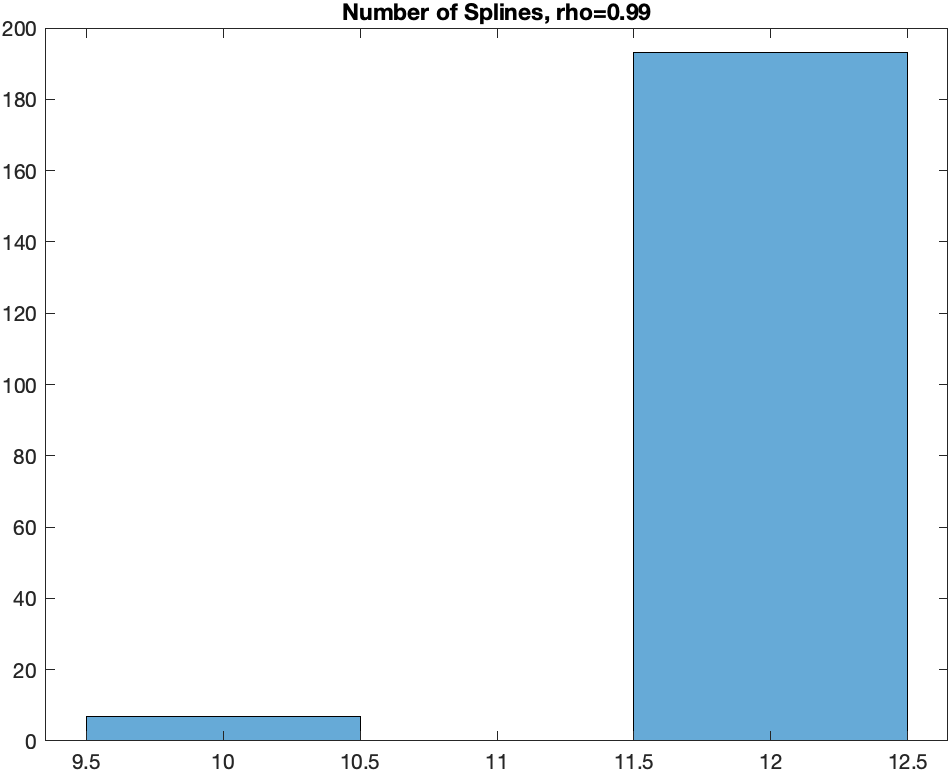
\includegraphics{../figures/hist_n_spli_rho-0.99_finer_grid.png}\end{minipage}%
%
\begin{minipage}{0.50\linewidth}
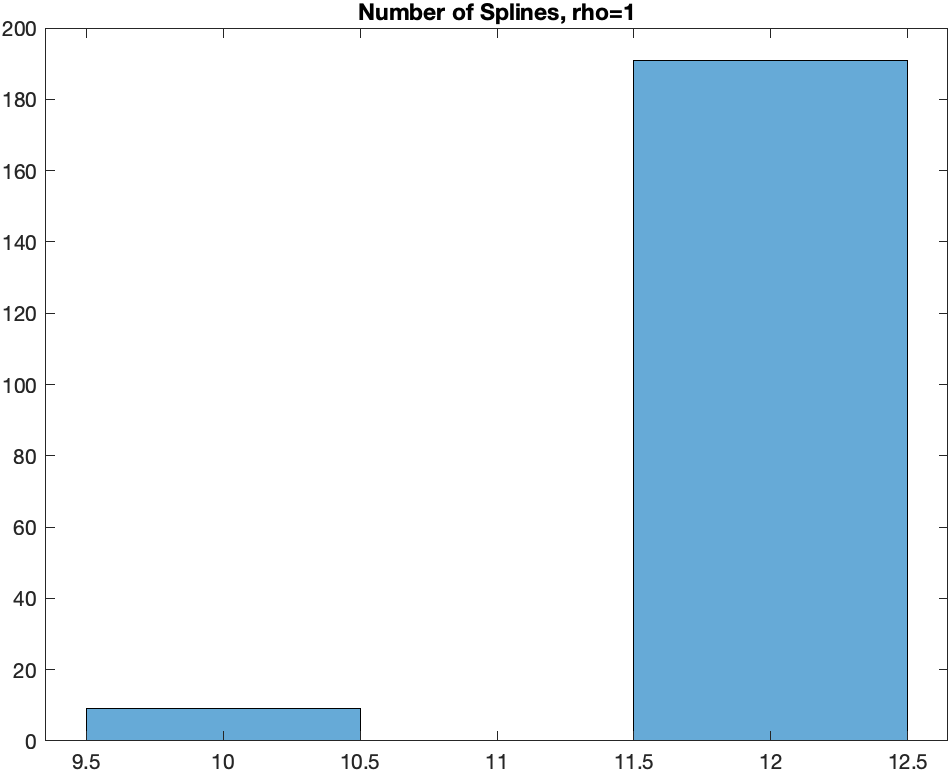
\includegraphics{../figures/hist_n_spli_rho-1_finer_grid.png}\end{minipage}%

\caption{\label{fig-hist-n-splies-finer-9}Histograms of the number of
quadratic B-splines chosen by the level of \(\rho\)}

\end{figure}%

\subsection*{References}\label{references}
\addcontentsline{toc}{subsection}{References}

\phantomsection\label{refs}
\begin{CSLReferences}{1}{0}
\bibitem[\citeproctext]{ref-Conley1999}
Conley, T G. 1999. {``GMM Estimation with Cross Sectional Dependence.''}
\emph{Journal of Econometrics} 92: 1--45.

\bibitem[\citeproctext]{ref-Hansen2020}
Hansen, Bruce E. 2020. \emph{ECONOMETRICS}.

\end{CSLReferences}



\end{document}
